\documentclass[a4paper,11pt,reqno]{amsart}

% --------------------------------------------------------
% Packages
% --------------------------------------------------------
\usepackage[utf8]{inputenc}
\usepackage[foot]{amsaddr}
\usepackage{amsmath,amsfonts,amssymb,amsthm,mathrsfs,bm}
\usepackage[margin=0.95in]{geometry}
\usepackage{color}
\usepackage[dvipsnames]{xcolor}
\usepackage{mathtools,graphicx}
\usepackage{tcolorbox}
\usepackage{listings}
\usepackage{textcomp}
\usepackage{units}
\usepackage{cite}
\usepackage{hyperref}
\usepackage{float}
\usepackage{overpic}
\usepackage{pgfplots}
\usepackage{subcaption} % 支持多图

% --------------------------------------------------------
% Custom Colours
% --------------------------------------------------------
\definecolor{CommentGreen}{rgb}{0.0,0.4,0.0}
\definecolor{Background}{rgb}{0.9,1.0,0.85}
\definecolor{lrow}{rgb}{0.914,0.918,0.922}
\definecolor{drow}{rgb}{0.725,0.745,0.769}
\definecolor{yellow-green}{rgb}{0.6, 0.8, 0.2}
\definecolor{brinkpink}{rgb}{0.98, 0.38, 0.5}
\definecolor{cornflowerblue}{rgb}{0.39, 0.58, 0.93}

% --------------------------------------------------------
% Typesetting Python code
% --------------------------------------------------------
\lstloadlanguages{Python}%
\lstset{
    language=Python, upquote=true, frame=single,
    basicstyle=\small\ttfamily,
    backgroundcolor=\color{yellow!30},
    keywordstyle=[1]\color{NavyBlue}\bfseries,
    keywordstyle=[2]\color{RubineRed},
    keywordstyle=[3]\color{orange!90}\bfseries,
    keywordstyle=[4]\color{Green!90}\bfseries,
    identifierstyle=,
    commentstyle=\usefont{T1}{pcr}{m}{sl}\color{MidnightBlue}\small,
    stringstyle=\color{purple},
    showstringspaces=false, tabsize=4, morekeywords={import,as},
    morekeywords=[2]{args,__init__},
    morekeywords=[3]{@property},
    morekeywords=[4]{self},
    morecomment=[l][\color{blue}]{...},
    numbers=none, firstnumber=1,
    numberstyle=\tiny\color{blue},
    stepnumber=1, xleftmargin=10pt, xrightmargin=10pt
}

\synctex=1

\hypersetup{
    unicode=false, pdftoolbar=true, 
    pdfmenubar=true, pdffitwindow=false, pdfstartview={FitH}, 
    pdftitle={ELE8088 Coursework}, pdfauthor={A. Author},
    pdfsubject={ELE8088 coursework}, pdfcreator={A. Author},
    pdfproducer={ELE8088}, pdfnewwindow=true,
    colorlinks=true, linkcolor=red,
    citecolor=blue, filecolor=magenta, urlcolor=cyan
}

% --------------------------------------------------------
% CUSTOM COMMANDS
% --------------------------------------------------------
\newcommand{\iu}{{\mathrm{i}\mkern1mu}}
\newcommand{\R}{{\rm I\!R}}
\newcommand{\N}{{\rm I\!N}}
\newcommand{\E}{{\rm I\!E}}
\newcommand{\C}{\mathbb{C}}
\newcommand{\dd}{\mathrm{d}}
\newcommand{\tran}{\intercal}
\DeclareMathOperator{\Var}{Var}
\DeclareMathOperator*{\argmin}{arg\,min}
\DeclareMathOperator*{\argmax}{arg\,max}
\DeclareMathOperator*{\minimise}{minimise}
\newcommand{\smallmat}[1]{\left[ \begin{smallmatrix}#1 \end{smallmatrix} \right]}
\newcommand{\smallplus}{{\scriptscriptstyle +}}
\newcommand{\Spp}{\mathbb{S}_{\smallplus\smallplus}}
\newcommand{\Sp}{\mathbb{S}_{\smallplus}}
\newcommand{\prob}{\mathrm{P}}
\renewcommand{\thefootnote}{\fnsymbol{footnote}}

% --------------------------------------------------------
% Opening: Title and Author Names
%          Modify this section
% --------------------------------------------------------
\title[ELE8088 Coursework]{Control \& Estimation Theory}

\author[Z. Zhang]{Zichi Zhang}
\author[S. Chen]{Shihao Chen}
\address[Zichi Zhang and Shihao Chen]{Email addresses: \href{mailto:zzhang54@qub.ac.uk}%
{zzhang54@qub.ac.uk} and 
\href{mailto:schen45.ac.uk}{schen45@qub.ac.uk}.}
\thanks{Thanks Dr. Pantelis Sopasakis. Version 1.1.9. Last updated:~\today.}



% --------------------------------------------------------
% Beginning of your document
% --------------------------------------------------------
\begin{document}

\maketitle

\vspace*{\fill}
\section*{\textbf{Collaboration Statement}}
    \noindent From the whole view, coursework Part I is divided into 3 parts which Zichi focused on the 1.1 and Shihao focused on the 1.2 then worked together on the 1.3.
    Of course, everyone has thought about all questions and proposed appropriate solutions. The above division of work is just to ensure that everyone has a focus.
    \\ \ \\
    Since the first time that Part I began, Zichi created a repository on GitHub and shared to Shihao immediately. Thus, we uploaded Python code and \LaTeX\ code, \LaTeX\ output and \LaTeX\ figures to the repository. Everyone uploaded his part on Python code and Zichi was responsible for the design of typing \LaTeX\ while both of us give our own opinions to make the PDF file looks more professional and closer to what Dr Pantelis Sopasakis shows on Canvas. For example, we have tried our best to plot similar figures and they are really much better than the past ones. It really cost us a lot of time on debugging every parameter including the gird and the color and thickness of every line.
    \\ \ \\
    On time management, we did not have an exact time to have a meet with each other but every time if anyone was trapped by a challenge for a long time then we would discuss it on the phone or have a Teams meeting to try to complete it and if both of the ways do not work that Zichi would ask Dr Pantelis Sopasakis for a possible hint. Besides this, we spent 8 hours every week on average and we had 5 face-to-face meetings to work these problems out. That was an efficient way when we got together and shared different ideas.
    \\ \ \\
    % Zichi really helped Shihao a lot on coding and knowledge of this course, Shihao needs to be more concentrated on the class that he can more easily work these questions out.
    % Also, Shihao made a plenty of ideas about the figures and his amazing imagination helped a lot.
    % \\ \ \\
    During this coursework, we both learned how to use GitHub and used Git commands in our coursework to commit changes. Since Dec. 2021, we totally created more than 15 commits in this repository, we try our best to make this collaborative project better with these useful tools.
    But in the same way, we still have a lot to improve, for example, we are biased in the division of labor. The difficulty of the three parts is not equal. Next time, we can better balance the difficulty of the two person. 
    Likewise, we need to strengthen our proficiency in coding and using various tools. We spent a lot of time getting familiar with these softwares in the beginning, and we can avoid these problems next time.
    \vspace*{\fill}
\newpage


% --------------------------------------------------------
% Section 1: Control
% --------------------------------------------------------
\section*{\Large\textbf{1\quad Part I: Control}}


% Subsection: Optimal Control
% ^^^^^^^^^^^^^^^^^^^^^^^^^^^
\subsection*{1.1\quad Optimal Control}\label{sec:q1}
\
\\ \\
(i) Prove that the function $g:\R^n\to \R$ given by $g(x) = \frac{1}{2}x^{\tran}Qx+q^{\tran}x+c$ with $Q\in \mathbb{S}^n_+$ is level-bounded
if and only if $Q\in \mathbb{S}^n_{++}$.
\\ 
\begin{proof}
    At first, we assume that $q^{\tran}=0$ and $c=0$. Then we have $g(x)=\tfrac{1}{2}x^{\tran}Qx$.
% \begin{align}
%     \mathrm{lev}_{\leq \alpha}g&=\{x\in\R^n:g(x)\leq\alpha\}
%     \\
%     &=\{x\in\R^n:\tfrac{1}{2}x^{\tran}Qx+q^{\tran}x+c\leq\alpha\}
% \end{align}
\begin{align}
    \mathrm{lev}_{\leq \alpha}g&=\{x\in\R^n:g(x)\leq\alpha\}
    \\
    &=\{x\in\R^n:x^{\tran}Qx\leq\alpha\}
\end{align}
We are trying to prove that $\mathrm{lev}_{\leq \alpha}g$ are bounded, i.e., there is an $M\geq 0$ such that
% \begin{equation}
%     \{x\in\R^n:\tfrac{1}{2}x^{\tran}Qx+q^{\tran}x+c\leq\alpha\}\subseteq \mathcal{B}_M
% \end{equation}
\begin{equation}
    \{x\in\R^n:\tfrac{1}{2}x^{\tran}Qx\leq\alpha\}\subseteq \mathcal{B}_M
    \label{eq:lev_prove_1}
\end{equation}
\begin{equation}
    \lambda_{\mathrm{min}}(Q)\left\lVert x\right\rVert ^2\leq \tfrac{1}{2}x^{\tran}Qx\leq \lambda_{\mathrm{max}}(Q)\left\lVert x\right\rVert ^2
    \label{eq:lev_prove_2}
\end{equation}
\begin{align}
    \Longrightarrow &\lambda_{\mathrm{min}}(Q)\left\lVert x\right\rVert ^2\leq \alpha
    \label{eq:lev_prove_3}
    \\
    \Longrightarrow &\left\lVert x\right\rVert \leq \sqrt{\frac{\alpha}{\lambda_{\mathrm{min}}(Q)}}=:M
    \label{eq:lev_prove_4}
\end{align}
Hence $g(x)=\tfrac{1}{2}x^{\tran}Qx$ is level-bounded if and only if $Q\in \mathbb{S}^n_{++}$.
\\
% \begin{equation}
%     \{x\in\R^n:x^{\tran}Qx\leq\alpha\}\subseteq \mathcal{B}_M
% \end{equation}
% \begin{equation}
%     \lambda_{\mathrm{min}}(Q)\left\lVert x\right\rVert ^2\leq x^{\tran}Qx\leq \lambda_{\mathrm{max}}(Q)\left\lVert x\right\rVert ^2
% \end{equation}
% \begin{align}
%     \Longrightarrow &\lambda_{\mathrm{min}}(Q)\left\lVert x\right\rVert ^2\leq \alpha\\
%     \Longrightarrow &\left\lVert x\right\rVert \leq \sqrt{\frac{\alpha}{\lambda_{\mathrm{min}}(Q)}}:=M
% \end{align}
% Thus, if $M\geq 0$ exists, then $\alpha\geq 0$, then
% \begin{align}
%     \lambda_{\mathrm{min}}(Q)\geq 0,\ &\lambda_{\mathrm{min}}(Q)\leq\lambda(Q)\leq\lambda_{\mathrm{max}}(Q)\\
%     \Longrightarrow&\lambda(Q)\geq 0\\
%     \Longrightarrow &Q\in \mathbb{S}^n_{++}
% \end{align}
Then, we try to prove the more general case, we know that from \emph{Exercise 21 (Completion of square) in handout X1}
\begin{align}
    x^{\tran}Qx-2b^{\tran}x=(x-Q^{-1}b)^{\tran}Q(x-Q^{-1}b)-b^{\tran}Q^{-1}b.
\end{align}
Then we have
\begin{align}
    \tfrac{1}{2}x^{\tran}Qx+q^{\tran}x+c=\tfrac{1}{2}\left( (x+Q^{-1}q)^{\tran}Q(x+Q^{-1}q)-q^{\tran}Q^{-1}q \right)+c .
\end{align}
% We can assume that
% \begin{align}
%     &-q^{\tran}Q^{-1}q + c=0
%     \\
%     \Longrightarrow &c=q^{\tran}Q^{-1}q
% \end{align}
% Thus, 
% \begin{align}
%     g(x)=\tfrac{1}{2} (x+Q^{-1}q)^{\tran}Q(x+Q^{-1}q)
% \end{align}
From \eqref{eq:lev_prove_1}\eqref{eq:lev_prove_2}\eqref{eq:lev_prove_3}\eqref{eq:lev_prove_4}, we can know that
\begin{align}
    g(x)=\tfrac{1}{2} (x+Q^{-1}q)^{\tran}Q(x+Q^{-1}q)
\end{align}
is level-bounded if and only if $Q\in \mathbb{S}^n_{++}$ at the same time to make sure $Q^{-1}$ exists, so $Q\in \Sp$.
\\
So if we plus a constant $-\tfrac{1}{2}q^{\tran}Q^{-1}q +c$
\begin{align}
    &g(x)=\tfrac{1}{2}\left( (x+Q^{-1}q)^{\tran}Q(x+Q^{-1}q)-q^{\tran}Q^{-1}q \right)+c
    \\
    &g(x)=\tfrac{1}{2}x^{\tran}Qx+q^{\tran}x+c
\end{align}
is level-bounded if and only if $Q\in \mathbb{S}^n_{++}$ at the same time to make sure $Q^{-1}$ exists, so $Q\in \Sp$.
Conclusion: the function $g:\R^n\to \R$ given by $g(x) = \frac{1}{2}x^{\tran}Qx+q^{\tran}x+c$ with $Q\in \mathbb{S}^n_+$ is level-bounded
if and only if $Q\in \mathbb{S}^n_{++}$.
\end{proof}
\
\\ \\
Next, consider the finite-horizon linear-quadratic optimal control problem
\begin{subequations}
    \begin{align}
        \mathbb{P}_N(x): \minimise_{\substack{u_0,u_1,\ldots,u_{N-1}\\ x_0,x_1,\ldots,x_N}} \,
         & \sum_{t=0}^{N-1}\textstyle\frac{1}{2}
         \begin{bmatrix}
             x_t\\
             u_t
         \end{bmatrix}^{\tran}
         \begin{bmatrix}
             Q&S\\
             S^{\tran}&R
         \end{bmatrix}
         \begin{bmatrix}
             x_t\\
             u_t
         \end{bmatrix}
         +\frac{1}{2}x_N^{\tran}P_fx_N,
        \\
        \text{subject to: }\,
         & x_{t+1} = A x_t + B u_t, \forall t\in\N_{[0, N-1]},
        \\
         & x_{0} = x,
    \end{align}
\end{subequations}
where $\begin{bsmallmatrix}Q&S\\S^{\tran}&R\end{bsmallmatrix}\succcurlyeq 0, Q\in \mathbb{S}^n_+, R\in \mathbb{S}^m_{++}, P_f\in \mathbb{S}^n_{+}$, and $x$ is a given initial state.
\\ \\
(ii) Is Problem $\mathbb{P}_N$ convex? Does $\mathbb{P}_N$ have a minimiser?
\\ \\
\textbf{Answer:}
% We can expand the problem $\mathbb{P}_N$:
% \begin{align}
%     \minimise_{\substack{u_0,u_1,\ldots,u_{N-1}\\ x_0,x_1,\ldots,x_N}} \,
%     & \sum_{t=0}^{N-1}\textstyle\frac{1}{2}
%          \begin{bmatrix}
%              x_t\\
%              u_t
%          \end{bmatrix}^{\tran}
%          \begin{bmatrix}
%              Q&S\\
%              S^{\tran}&R
%          \end{bmatrix}
%          \begin{bmatrix}
%              x_t\\
%              u_t
%          \end{bmatrix}
%          +\frac{1}{2}x_N^{\tran}P_fx_N,
%     \\
%     =\minimise_{\substack{u_0,u_1,\ldots,u_{N-1}\\ x_0,x_1,\ldots,x_N}} \,
%     &\sum_{t=0}^{N-1}\textstyle\frac{1}{2}
%     (x_t^{\tran}Qx_t+u_t^{\tran}Ru_t+x_t^{\tran}Su_t+u_t^{\tran}S^{\tran}x_t
%     +x_N^{\tran}P_fx_N),
% \end{align}
From \textit{Theorem (Second-order differentiability and convexity)}
\begin{align}
    &Let\ f : \R^n\rightarrow\R\ be\ \mathcal{C}^2.\ Then\ f\ is\ convex\ if\ and\ only\ if
    \notag
    \\
    &\qquad\qquad\qquad\qquad\qquad \nabla ^2f(x)\succeq   0,
    \\
    &for\ all\ x \in\R^n.
    \notag
\end{align}
Thus, we have
\begin{equation}
    \nabla ^2(\mathbb{P}_N)=
    \begin{bmatrix}
        Q&S\\
        S^{\tran}&R
    \end{bmatrix}
\end{equation}
It is convex iff $\begin{bsmallmatrix}Q&S\\S^{\tran}&R\end{bsmallmatrix}\succeq 0$.
\\
And we know that $\begin{bsmallmatrix}Q&S\\S^{\tran}&R\end{bsmallmatrix}\succcurlyeq 0, Q\in \mathbb{S}^n_+, R\in \mathbb{S}^m_{++}, P_f\in \mathbb{S}^n_{+}$. So the function in problem $\mathbb{P}_N$ is convex. 
\\
And $\mathbb{P}_N$ is an optimization problem in which the objective function is a convex function and the feasible set is a convex set $\R^n$.
Also the constraints $x_{t+1}=Ax_t+Bu_t,\ x_0=x$ are convex.
\\
\textbf{So problem $\mathbb{P}_N$ is convex.}
\\ \\
From \textit{Proposition (Minimisers of $\mathcal{C}^1$ convex functions)}
\begin{align}
    &Let\ f : \R^n\rightarrow\R\ be\ a\ convex\ and\ \mathcal{C}^1\ function.\ Then
    \notag
    \\
    &the\ set\ of\ stationary\ points\ of\ f\ is\ equal\ to\ \argmin f.
    \notag
    \\
    &In\ other\ words,\ a\ point\ x^{\star}\in\R^n\ is\ a\ minimiser\ of\ f\ 
    \notag
    \\
    &if\ and\ only\ if\ it\ is\ a\ stationary\ point.
    \notag
\end{align}
We know that $\mathbb{P}_N$ is convex, therefore all stationary
points of $\mathbb{P}_N$ are minimisers of the problem \textit{(Proposition (Minimisers of $\mathcal{C}^1$ convex functions))}.
\\
It is 
\begin{align}
    &\quad \ \nabla (\mathbb{P}_N(x^{\star},u^{\star}))
    \\
    &=\nabla \left(
        \minimise_{\substack{u^{\star}_0,u^{\star}_1,\ldots,u^{\star}_{N-1}\\ x^{\star}_0,x^{\star}_1,\ldots,x^{\star}_N}} \,
        \sum_{t=0}^{N-1}\tfrac{1}{2}
        \begin{bmatrix}
            x_t\\
            u_t
        \end{bmatrix}^{\tran}
        \begin{bmatrix}
            Q&S\\
            S^{\tran}&R
        \end{bmatrix}
        \begin{bmatrix}
            x_t\\
            u_t
        \end{bmatrix}
        +\tfrac{1}{2}x_N^{\tran}P_fx_N\right) 
    \\
    &= 0
    \\
    &\Longleftrightarrow 
    \minimise_{\substack{u^{\star}_0,u^{\star}_1,\ldots,u^{\star}_{N-1}\\ x^{\star}_0,x^{\star}_1,\ldots,x^{\star}_N}} \,
    \sum_{t=0}^{N-1}
    \begin{bmatrix}
        Q&S\\
        S^{\tran}&R
    \end{bmatrix}
    \begin{bmatrix}
        x_t\\
        u_t
    \end{bmatrix}
    +P_fx_N
    \label{eq:P_N_minimiser}
\end{align}
Any point $x^{\star},\ u^{\star}$ that satisfies the Equation \eqref{eq:P_N_minimiser} is a minimiser of $\mathbb{P}_N$.
\\
\textbf{So problem $\mathbb{P}_N$ has a minimiser.}
\\ \\
(iii) Solve Problem $\mathbb{P}_N$ by eliminating the state sequence: determine the optimal sequence of control actions, the optimal sequence(s) of states and the optimal cost.
\\ \\
\textbf{Solusion:}
\begin{subequations}
    \begin{align}
        \mathbb{P}_N(x): \minimise_{\substack{u_0,u_1,\ldots,u_{N-1}\\ x_0,x_1,\ldots,x_N}} \,
         & \sum_{t=0}^{N-1}\textstyle\frac{1}{2}
         \begin{bmatrix}
             x_t\\
             u_t
         \end{bmatrix}^{\tran}
         \begin{bmatrix}
             Q&S\\
             S^{\tran}&R
         \end{bmatrix}
         \begin{bmatrix}
             x_t\\
             u_t
         \end{bmatrix}
         +\frac{1}{2}x_N^{\tran}P_fx_N,
        \\
        \text{subject to: }\,
         & x_{t+1} = A x_t + B u_t, \forall t\in\N_{[0, N-1]},
        \\
         & x_{0} = x,
    \end{align}
\end{subequations}
where $\begin{bsmallmatrix}Q&S\\S^{\tran}&R\end{bsmallmatrix}\succcurlyeq 0, Q\in \mathbb{S}^n_+, R\in \mathbb{S}^m_{++}, P_f\in \mathbb{S}^n_{+}$, and $x$ is a given initial state.
\\
Given $x_{0} = x$, we have
\begin{subequations}
    \begin{align}
        x_1&=Ax+Bu_0
        \\
        x_2&=Ax_1+Bu_1
        \\
        &=A^2x+ABu_0+Bu_1
        \\
        x_3&=Ax_2+Bu_2
        \\
        &=A^3x+A^2Bu_0+ABu_1+Bu_2
        \\
        &\ \, \vdots 
        \\
        x_t&=A^{t}x+A^{t-1}Bu_0+\ldots +Bu_{t-1}.
    \end{align}
\end{subequations}
Let us define $\bm{x}_N = (x_1, x_2,\ldots, x_N)$ and $\bm{u}_N = (u_0,\ldots, u_{N-1})$; then,
\begin{equation}
    \bm{x}=\bar{A}x+\bar{B}\bm{u}_N,
\end{equation}
where
\begin{equation}
    \bar{A}=
    \begin{bmatrix}
        A
        \\
        A^2
        \\
        A^3
        \\
        \vdots
        \\
        A^N
    \end{bmatrix},
    \bar{B}=
    \begin{bmatrix}
        B
        \\
        AB&B
        \\
        A^2B&AB&B
        \\
        A^3B&A^2B&AB&B
        \\
        \vdots&\vdots&\vdots&&\ddots
        % \\
        % \vdots&\vdots&\vdots&&&B
        \\
        A^NB&A^{N-1}B&\cdots&&AB&B
    \end{bmatrix}
\end{equation}
By defining
\begin{equation}
    \bar{Q}=\mathrm{blkdiag}(Q_1,Q_2,\ldots,Q_{N-1},P_f),\ \text{and}\ \bar{R}=\mathrm{blkdiag}(R_1,R_2,\ldots,R_{N-1}),
\end{equation}
and omitting the constant $\tfrac{1}{2}
\begin{bsmallmatrix}
    x_0\\
    u_0
\end{bsmallmatrix}^{\tran}
\begin{bsmallmatrix}
    \bar{Q}&S\\
    S^{\tran}&\bar{R}
\end{bsmallmatrix}
\begin{bsmallmatrix}
    x_0\\
    u_0
\end{bsmallmatrix}$ from the cost, $\mathbb{P}_N$ can be written equivalently as
\begin{subequations}
    \begin{align}
        \mathbb{P}_N(x): \minimise_{\bm{u_N},\bm{x_N}} \,
        & \tfrac{1}{2}
        \begin{bmatrix}
            \bm{x}_N\\
            \bm{u}_N
        \end{bmatrix}^{\tran}
        \begin{bmatrix}
            \bar{Q}&S\\
            S^{\tran}&\bar{R}
        \end{bmatrix}
        \begin{bmatrix}
            \bm{x}_N\\
            \bm{u}_N
        \end{bmatrix},
        \\
        \text{subject to: }\,
        & \bm{x}_{N} = \bar{A} x + \bar{B} \bm{u}_N,
        \\
        & x_{0} = x,
    \end{align}
\end{subequations}
and substituting the constraints into the cost function we obtain the unconstrained problem:
\begin{subequations}
    \begin{align}
        \mathbb{P}_N(x): \minimise_{\bm{u_N}} \,
        & \tfrac{1}{2}
        \begin{bmatrix}
            \bar{A} x + \bar{B}\bm{u}_N\\
            \bm{u}_N
        \end{bmatrix}^{\tran}
        \begin{bmatrix}
            \bar{Q}&S\\
            S^{\tran}&\bar{R}
        \end{bmatrix}
        \begin{bmatrix}
            \bar{A} x + \bar{B}\bm{u}_N\\
            \bm{u}_N
        \end{bmatrix},
        \\
        &=\tfrac{1}{2}\left((\bar{A}x + \bar{B}\bm{u}_N)^{\tran}\bar{Q}(\bar{A} x + \bar{B}\bm{u}_N)+\bm{u}_N^{\tran}\bar{R}\bm{u}_N\right.
        \\
        &\left.\quad+(\bar{A}x + \bar{B}\bm{u}_N)^{\tran}S\bm{u}_N+\bm{u}_N^{\tran}S^{\tran}(\bar{A} x + \bar{B}\bm{u}_N)\right) 
        \\
        &=\tfrac{1}{2}\left((\bar{A}x)^{\tran}\bar{Q}\bar{A}x+(\bar{A}x)^{\tran}\bar{Q}\bar{B}\bm{u}_N+(\bar{B}\bm{u}_N)^{\tran}\bar{Q}\bar{A}x\right.
        \\
        &\quad+(\bar{B}\bm{u}_N)^{\tran}\bar{Q}\bar{B}\bm{u}_N+\bm{u}_N^{\tran}\bar{R}\bm{u}_N+(\bar{A}x)^{\tran}S\bm{u}_N
        \\
        &\left.\quad+(\bar{B}\bm{u}_N)^{\tran}S\bm{u}_N+\bm{u}_N^{\tran}S^{\tran}\bar{A}x+\bm{u}_N^{\tran}S^{\tran}\bar{B}\bm{u}_N\right) 
    \end{align}
\end{subequations}
If we expand the cost function and drop the constant term $(\bar{A}x)^{\tran}\bar{Q}\bar{A}x$, we obtain:
\begin{subequations}
    \begin{align}
        \mathbb{P}_N(x): \minimise_{\bm{u_N}} \,
        &\tfrac{1}{2}\left((\bar{A}x)^{\tran}\bar{Q}\bar{B}\bm{u}_N+(\bar{B}\bm{u}_N)^{\tran}\bar{Q}\bar{A}x\right.
        \\
        &\quad+(\bar{B}\bm{u}_N)^{\tran}\bar{Q}\bar{B}\bm{u}_N+\bm{u}_N^{\tran}\bar{R}\bm{u}_N+(\bar{A}x)^{\tran}S\bm{u}_N 
        \\
        &\left.\quad+(\bar{B}\bm{u}_N)^{\tran}S\bm{u}_N+\bm{u}_N^{\tran}S^{\tran}\bar{A}x+\bm{u}_N^{\tran}S^{\tran}\bar{B}\bm{u}_N \right) 
        \\
        &=\tfrac{1}{2}\left( (\bar{A}x)^{\tran}(\bar{Q}\bar{B}+S)\bm{u}_N+\bm{u}_N^{\tran}(\bar{B}^{\tran}\bar{Q}+S^{\tran})\bar{A}x\right.
        \\
        &\left.\quad+\bm{u}_N^{\tran}(\bar{B}^{\tran}\bar{Q}\bar{B}+\bar{R}+\bar{B}^{\tran}S+S^{\tran}\bar{B})\bm{u}_N \right)
        \\
        &=\tfrac{1}{2}\bm{u}_N^{\tran}(\bar{R}+\bar{B}^{\tran}\bar{Q}\bar{B}+\bar{B}^{\tran}S+S^{\tran}\bar{B})\bm{u}_N
        \\
        &\quad+(\bar{B}^{\tran}\bar{Q}\bar{A}x+S^{\tran}\bar{A}x)^{\tran}\bm{u}_N
    \end{align}
\end{subequations}
This is a quadratic optimisation problem with Hessian
$\bar{R}+\bar{B}^{\tran}\bar{Q}\bar{B}+\bar{B}^{\tran}S+S^{\tran}\bar{B}$.
Recall that $\begin{bsmallmatrix}Q&S\\S^{\tran}&R\end{bsmallmatrix}\succcurlyeq 0, Q\in \mathbb{S}^n_+, R\in \mathbb{S}^m_{++}, P_f\in \mathbb{S}^n_{+}$.
As a result, $\bar{Q}\in\Sp^{Nn},\ R\in\Spp^{Nm}$ and
$\bar{R}+\bar{B}^{\tran}\bar{Q}\bar{B}+\bar{B}^{\tran}S+S^{\tran}\bar{B}\in\Spp^{Nm}$
and $\mathbb{P}_N(x)$ is a convex optimisation problem.
A $\bm{u}_N^{\star}$ is a minimiser iff
$(\bar{R}+\bar{B}^{\tran}\bar{Q}\bar{B}+\bar{B}^{\tran}S+S^{\tran}\bar{B})\bm{u}_N^{\star}+\bar{B}^{\tran}\bar{Q}\bar{A}x+S^{\tran}\bar{A}x=0$
and the problem has the unique solution:
\begin{equation}
    \bm{u}_N^{\star}=-(\bar{R}+\bar{B}^{\tran}\bar{Q}\bar{B}+\bar{B}^{\tran}S+S^{\tran}\bar{B})^{-1}(\bar{B}^{\tran}\bar{Q}\bar{A}x+S^{\tran}\bar{A}x)
\end{equation}
\
\\ \\
(iv) Solve Problem $\mathbb{P}_N$ by using the dynamic programming method.
\\ \\
\textbf{Solusion:}
We can expand the problem $\mathbb{P}_N$ and add two items and then rearrange it:
\begin{align}
    \minimise_{\substack{u_0,u_1,\ldots,u_{N-1}\\ x_0,x_1,\ldots,x_N}} \,
    & \sum_{t=0}^{N-1}\textstyle\frac{1}{2}
    \begin{bmatrix}
        x_t\\
        u_t
    \end{bmatrix}^{\tran}
    \begin{bmatrix}
        Q&S\\
        S^{\tran}&R
    \end{bmatrix}
    \begin{bmatrix}
        x_t\\
        u_t
    \end{bmatrix}+\tfrac{1}{2}x_N^{\tran}P_fx_N
    \\
    =\minimise_{\substack{u_0,u_1,\ldots,u_{N-1}\\ x_0,x_1,\ldots,x_N}} \,
    &\sum_{t=0}^{N-1}\textstyle\frac{1}{2}
    (x_t^{\tran}Qx_t+u_t^{\tran}Ru_t+x_t^{\tran}Su_t+u_t^{\tran}S^{\tran}x_t
    +x_N^{\tran}P_fx_N)
    \\
    =\minimise_{\substack{u_0,u_1,\ldots,u_{N-1}\\ x_0,x_1,\ldots,x_N}} \,
    &\sum_{t=0}^{N-1}\textstyle\frac{1}{2}
    (\underbracket[0.5pt]{x_t^{\tran}Qx_t+u_t^{\tran}Ru_t+x_t^{\tran}Su_t+u_t^{\tran}S^{\tran}x_t}_{\text{original items}}
    +\underbracket[0.5pt]{x_t^{\tran}SR^{-1}S^{\tran}x_t-x_t^{\tran}SR^{-1}S^{\tran}x_t}_{\text{added items}}
    \\
    &\qquad+x_N^{\tran}P_fx_N)
    \\
    =\minimise_{\substack{u_0,u_1,\ldots,u_{N-1}\\ x_0,x_1,\ldots,x_N}} \,
    &\sum_{t=0}^{N-1}\textstyle\frac{1}{2}
    (\underbracket[0.5pt]{x_t^{\tran}(Q-SR^{-1}S^{\tran})x_t}_{\text{PartA}}+\underbracket[0.5pt]{(u_t+R^{-1}S^{\tran}x_t)^{\tran}R(u_t+R^{-1}S^{\tran}x_t)}_{\text{PartB}}
    \\
    &\qquad+x_N^{\tran}P_fx_N)
    \label{eq:P_N_matrix_rewrite}
\end{align}
\begin{align}
    \mathrm{PartA}&=x_t^{\tran}Qx_t-x_t^{\tran}SR^{-1}S^{\tran}x_t
    \\
    &=x_t^{\tran}(Q-SR^{-1}S^{\tran})x_t
    \\
    \mathrm{PartB}&=u_t^{\tran}Ru_t+x_t^{\tran}Su_t+u_t^{\tran}S^{\tran}x_t+x_t^{\tran}SR^{-1}S^{\tran}x_t
    \\
    &=u_t^{\tran}Ru_t+x_t^{\tran}S\!\!\!\!\!\!\underbracket[0.5pt]{R^{-1}R}_{\text{added items}}\!\!\!\!\!u_t+u_t^{\tran}\!\!\!\!\!\!\underbracket[0.5pt]{RR^{-1}}_{\text{added items}}\!\!\!\!\!S^{\tran}x_t+x_t^{\tran}S\!\!\!\!\!\!\underbracket[0.5pt]{R^{-1}R}_{\text{added items}}\!\!\!\!\!R^{-1}S^{\tran}x_t
    \\
    &=(u_t^{\tran}+x_t^{\tran}SR^{-1})R(u_t+R^{-1}S^{\tran}x_t)
    \\
    &=(u_t+R^{-1}S^{\tran}x_t)^{\tran}R(u_t+R^{-1}S^{\tran}x_t)
\end{align}
Let
\begin{equation}
    \begin{cases}
        \tilde{Q}=Q-SR^{-1}S^{\tran}\\
        \tilde{u}_t=u_t+R^{-1}S^{\tran}x_t
    \end{cases}
    \label{eq:tilde_Q_u}
\end{equation}
\begin{align}
    x_{t+1}&=Ax+B(\tilde{u}_t-R^{-1}S^{\tran}x_t)\notag\\
    &=(A-BR^{-1}S^{\tran})x_t+B\tilde{u}_t, \forall t\in\N_{[0, N-1]}
    \label{eq:tilde_x}
\end{align}
Let
\begin{equation}
    \tilde{A}=A-BR^{-1}S^{\tran}
    \label{eq:tilde_A}
\end{equation}
The problem changes to 
\begin{subequations}
    \begin{align}
        \mathbb{P}_N(x): \minimise_{\substack{u_0,u_1,\ldots,u_{N-1}\\ x_0,x_1,\ldots,x_N}} \,
         & \sum_{t=0}^{N-1}\left(\tfrac{1}{2}
         x_t^{\tran}\tilde{Q}x_t+\tilde{u}_t^{\tran}R\tilde{u}_t\right) 
         +\tfrac{1}{2}x_N^{\tran}P_fx_N,
        \\
        \text{subject to: }\,
         & x_{t+1} = \tilde{A}x_t+B\tilde{u}_t, \forall t\in\N_{[0, N-1]},
        \\
         & x_{0} = x,
    \end{align}
\end{subequations}
where $Q\in \mathbb{S}^n_+, R\in \mathbb{S}^m_{++}, P_f\in \mathbb{S}^n_{+}, \tilde{Q}=Q-SR^{-1}S^{\tran}, \tilde{u}_t=u_t+R^{-1}S^{\tran}x_t, \tilde{A}=A-BR^{-1}S^{\tran}$, and $x$ is a given initial state.
\\ \\
We identify the terminal cost, the stage cost, and the system dynamics. We have
\begin{align}
    V_f(x)&=\textstyle\frac{1}{2}x^{\tran}P_fx,\\
    \ell(x,\tilde{u})&=\textstyle\frac{1}{2}x^{\tran}\tilde{Q}x+\tilde{u}^{\tran}R\tilde{u},\\
    f(x,\tilde{u})&=\tilde{A}x+B\tilde{u}.
\end{align}
We define $V_{0}^{\star}(x)=V_f(x)$, i.e.,
\begin{equation}
    V_{0}^{\star}(x)=\textstyle\frac{1}{2}x^{\tran}P_fx.
\end{equation}
Then, we know that $V_{t+1}^{\star}(x)=(\mathbb{T}V_t^{\star})(x)$. We assume that
\begin{equation}
    V_t^{\star}(x)=\textstyle\frac{1}{2}x^{\tran}P_tx.
\end{equation}
We have
\begin{align} 
    V_t^{\star}(x)&=(\mathbb{T}V_t^{\star})(x)=\min_{\tilde{u}}\left\{\ell(x,\tilde{u})+V_t^{\star}(f(x,\tilde{u}))\right\} \notag\\
    &=\min_{\tilde{u}}\left\{\textstyle\frac{1}{2}x^{\tran}\tilde{Q}x+\tilde{u}^{\tran}R\tilde{u}+\frac{1}{2}(\tilde{A}x+B\tilde{u})^{\tran}P_t(\tilde{A}x+B\tilde{u})\right\}.
\end{align}
After some algebraic manipulations
\begin{equation}
    V_{t+1}^{\star}(x)=\textstyle\frac{1}{2}x^{\tran}(\tilde{Q}+\tilde{A}^{\tran}P_t\tilde{A})x+\min_{\tilde{u}}\left\{\textstyle\frac{1}{2}\tilde{u}^{\tran}(R+B^{\tran}P_tB)\tilde{u}+(B^{\tran}P_t\tilde{A}x)^{\tran}\tilde{u}\right\}.
    \label{eq:V_t+1(x)}
\end{equation}
The minimiser is...
\begin{equation}
    \kappa_{t+1}^{\star}(x)=-(R+B^{\tran}P_tB)^{-1}B^{\tran}P_tAx.
\end{equation}
It is convenient to write $\kappa^{\star}_{t+1}$ as an affine function, i.e., $\kappa_{t+1}^{\star}(x)=K_{t+1}x$, where $K_{t+1}$ is given by
\begin{equation}
    K_{t+1}=-(R+B^{\tran}P_tB)^{-1}B^{\tran}P_tA.
\end{equation}
We can then substitute $\tilde{u}=\kappa_{t+1}^{\star}$ in Equation \eqref{eq:V_t+1(x)}:
\begin{align}
    V_{t+1}^{\star}(x)&=\textstyle\frac{1}{2}x^{\tran}(\tilde{Q}+\tilde{A}^{\tran}P_t\tilde{A})x+\min_{\tilde{u}}\left\{\textstyle\frac{1}{2}\tilde{u}^{\tran}(R+B^{\tran}P_tB)\tilde{u}+(B^{\tran}P_t\tilde{A}x)^{\tran}\tilde{u}\right\}\notag\\
    &=\textstyle\frac{1}{2}x^{\tran}(\tilde{Q}+\tilde{A}^{\tran}P_t\tilde{A})x+\frac{1}{2}(K_{t+1}x)^{\tran}(R+B^{\tran}P_tB)(K_{t+1}x)+(B^{\tran}P_t\tilde{A}x)^{\tran}(K_{t+1}x).
\end{align}
and we can rearrange the terms to write $V_{t+1}^{\star}$ in the form $V_{t+1}^{\star}(x)=\textstyle\frac{1}{2}x^{\tran}P_{t+1}x$.\\
We find that
\begin{equation}
    P_{t+1}=\tilde{Q}+\tilde{A}^{\tran}P_t\tilde{A}+K_{t+1}^{\tran}(R_t+B^{\tran}P_tB)K_{t+1}+2\tilde{A}^{\tran}P_t^{\tran}BK_{t+1}.
\end{equation}
We have that
\begin{equation}
    V_{N}^{\star}(x)=\textstyle\frac{1}{2}x^{\tran}P_Nx.
\end{equation}
We have
\begin{align}
    x_0^{\star}=&x,\notag\\
    \tilde{u}_0^{\star}=&\kappa_N^{\star}(x_0^{\star})=K_Nx_0^{\star},\notag\\
    x_1^{\star}=&\tilde{A}x_0^{\star}+B\tilde{u}_0^{\star},\notag\\
    \tilde{u}_1^{\star}=&\kappa_{N-1}^{\star}(x_1^{\star})=K_{N-1}x_1^{\star},\notag\\
    x_2^{\star}=&\tilde{A}x_1^{\star}+B\tilde{u}_1^{\star},\notag\\
    &\vdots \notag\\
    \tilde{u}_{N-1}^{\star}=&\kappa_1^{\star}(x_{N-1}^{\star})=K_1x_{N-1}^{\star},\notag\\
    x_N^{\star}=&\tilde{A}x_{N-1}^{\star}+B\tilde{u}_{N-1}^{\star}.\notag
\end{align}
Finally, we get the solutions by using the dynamic programming method.
\\ \\ \\
Next, consider the following infinite-horizon optimal control problem
\begin{subequations}
    \begin{align}
        \mathbb{P}_{\infty}(x): \minimise_{(u_t)_{t\in \N},(x_t)_{t\in \N}} \,
        & \sum_{t=0}^{\infty}\textstyle\frac{1}{2}
        \begin{bmatrix}
            x_t\\
            u_t
        \end{bmatrix}^{\tran}
        \begin{bmatrix}
            Q&S\\
            S^{\tran}&R
        \end{bmatrix}
        \begin{bmatrix}
            x_t\\
            u_t
        \end{bmatrix},
        \\
        \text{subject to: }\,
        & x_{t+1} = A x_t + B u_t, t\in\N,
        \\
        & x_{0} = x,
    \end{align}
\end{subequations}
where $\begin{bsmallmatrix}Q&S\\S^{\tran}&R\end{bsmallmatrix}\succcurlyeq 0, Q\in \mathbb{S}^n_+, R\in \mathbb{S}^m_{++}$.
\\ \\
(v) Under what conditions do the dynamic programming iterates, $V^{\star}_t$, converge? Justify your answer.
\\ \\
\textbf{Anwser:} In order for the dynamic programming iterates, $V^{\star}_t$, converge, it is necessary that there is a sequence of inputs $(u_t)_{t\in \N}$, such that the corresponding states, $(x_t)_{t\in \N}$, are such that the cost function is finite
\begin{equation}
    \sum_{t=0}^{\infty}\textstyle\frac{1}{2}
        \begin{bmatrix}
            x_t\\
            u_t
        \end{bmatrix}^{\tran}
        \begin{bmatrix}
            Q&S\\
            S^{\tran}&R
        \end{bmatrix}
        \begin{bmatrix}
            x_t\\
            u_t
        \end{bmatrix}
    <\infty
\end{equation}
We denote the value function of $\mathbb{P}_{\infty}(x)$ by $V_{\infty}^{\star}(x)$, that is
\begin{equation}
    V_{\infty}^{\star}(x)=\inf_{(u_t)_{t\in \N},(x_t)_{t\in \N}}
    \left\{
    \sum_{t=0}^{\infty}\tfrac{1}{2}
        \begin{bmatrix}
            x_t\\
            u_t
        \end{bmatrix}^{\tran}
        \begin{bmatrix}
            Q&S\\
            S^{\tran}&R
        \end{bmatrix}
        \begin{bmatrix}
            x_t\\
            u_t
        \end{bmatrix}
        \left\lvert
            x_{t+1}=Ax_t+Bu_t,\forall t\in\N,\atop
            x_0=x
        \right. 
    \right\} 
\end{equation}
The value function $V^{\star}_{\infty}$, if it exists, must satisfy $V^{\star}_{\infty}=\mathbb{T}V^{\star}_{\infty}$, which can be equivalently written as
\begin{equation}
    V_{\infty}^{\star}(x)=\min_u
    \left\{
    \sum_{t=0}^{\infty}\tfrac{1}{2}
        \begin{bmatrix}
            x_t\\
            u_t
        \end{bmatrix}^{\tran}
        \begin{bmatrix}
            Q&S\\
            S^{\tran}&R
        \end{bmatrix}
        \begin{bmatrix}
            x_t\\
            u_t
        \end{bmatrix}
        +V_{\infty}^{\star}(x)(Ax+Bu)
    \right\} 
\end{equation}
By Equations \eqref{eq:P_N_matrix_rewrite}, \eqref{eq:tilde_Q_u}, \eqref{eq:tilde_x} and \eqref{eq:tilde_A}, the problem changes to 
\begin{subequations}
    \begin{align}
        \mathbb{P}_{\infty}(x): \minimise_{(u_t)_{t\in \N},(x_t)_{t\in \N}} \,
         & \sum_{t=0}^{\infty}\left(\textstyle\frac{1}{2}
         x_t^{\tran}\tilde{Q}x_t+\tilde{u}_t^{\tran}R\tilde{u}_t\right),
        \\
        \text{subject to: }\,
         & x_{t+1} = \tilde{A}x_t+B\tilde{u}_t, t\in\N,
        \\
         & x_{0} = x,
    \end{align}
\end{subequations}
where $Q\in \mathbb{S}^n_+, R\in \mathbb{S}^m_{++}, \tilde{Q}=Q-SR^{-1}S^{\tran}, \tilde{u}_t=u_t+R^{-1}S^{\tran}x_t, \tilde{A}=A-BR^{-1}S^{\tran}$.
\\ \\
We have known a matrix $P$ satisfying
\begin{equation}
    P=Q+A^{\tran}(P-PB(R+B^{\tran}PB)^{-1}B^{\tran}P)A,
    \tag{DARE}
    \label{eq:DARE}
\end{equation}
which is known a \emph{discrete algebraic Riccati equation} \eqref{eq:DARE}, and
\begin{equation}
    V^{\star}_{\infty}=\tfrac{1}{2}x^{\tran}Px.
\end{equation}
In $\mathbb{P}_{\infty}(x)$, we have
\begin{equation}
    P=\tilde{Q}+\tilde{A}^{\tran}(P-PB(R+B^{\tran}PB)^{-1}B^{\tran}P)\tilde{A}.
    \label{eq:P_N}
\end{equation}
where $Q\in \mathbb{S}^n_+, R\in \mathbb{S}^m_{++}, \tilde{Q}=Q-SR^{-1}S^{\tran}, \tilde{A}=A-BR^{-1}S^{\tran}$.
\\ \\
In those conditions, the dynamic programming iterates, $V^{\star}_t$, converge
\begin{equation}
    \lim_{t\to\infty}V^{\star}_{t}=\tfrac{1}{2}x_t^{\tran}Px_t.
\end{equation}
\
\\
(vi) Prove that the optimal value of $\mathbb{P}_{\infty}(x)$, if it exists, is given by $V(x)=\frac{1}{2}x^{\tran}Px$ where $P\in \mathbb{S}^n_{++}$ Snsatisfies the algebraic equation
\begin{equation}
    P=A^{\tran}PA-(A^{\tran}PB+S)(R+B^{\tran}PB)^{-1}(B^{\tran}PA+S^{\tran})+Q.
    \label{eq:P}
\end{equation}
\\
\begin{proof}
In $\mathbb{P}_{\infty}(x)$, we have
\begin{equation}
    P=\tilde{Q}+\tilde{A}^{\tran}(P-PB(R+B^{\tran}PB)^{-1}B^{\tran}P)\tilde{A}.
\end{equation}
where $Q\in \mathbb{S}^n_+, R\in \mathbb{S}^m_{++}, \tilde{Q}=Q-SR^{-1}S^{\tran}, \tilde{A}=A-BR^{-1}S^{\tran}$.
\\
We try to expanding Equation \eqref{eq:P_N}:
\begin{align}
    P&=\tilde{Q}+\tilde{A}^{\tran}(P-PB(R+B^{\tran}PB)^{-1}B^{\tran}P)\tilde{A}
    \\
    &=Q-SR^{-1}S^{\tran}+(A-BR^{-1}S^{\tran})^{\tran}(P-PB(R+B^{\tran}PB)^{-1}B^{\tran}P)(A-BR^{-1}S^{\tran})
    \\
    &=Q-SR^{-1}S^{\tran}+(A^{\tran}-SR^{-1}B^{\tran})(P-PB(R+B^{\tran}PB)^{-1}B^{\tran}P)(A-BR^{-1}S^{\tran})
    \\
    &=Q-SR^{-1}S^{\tran}+A^{\tran}PA-A^{\tran}PBR^{-1}S^{\tran}-SR^{-1}B^{\tran}PA+SR^{-1}B^{\tran}PBR^{-1}S^{\tran}
    \\
    &\quad-A^{\tran}PB(R+B^{\tran}PB)^{-1}B^{\tran}PA+A^{\tran}PB(R+B^{\tran}PB)^{-1}B^{\tran}PBR^{-1}S^{\tran}
    \\
    &\quad+SR^{-1}B^{\tran}PB(R+B^{\tran}PB)^{-1}B^{\tran}PA-SR^{-1}B^{\tran}PB(R+B^{\tran}PB)^{-1}B^{\tran}PBR^{-1}S^{\tran}
    \\
    &=Q+A^{\tran}PA-(A^{\tran}PB+S)(R+B^{\tran}PB)^{-1}(B^{\tran}PA+S^{\tran})
    % \\
    % &=Q+A^{\tran}PA+S(R^{-1}+R^{-1}B^{\tran}PB(R+B^{\tran}PB)^{-1}B^{\tran}PBR^{-1})S^{\tran}
\end{align}
Thus, the optimal value of $\mathbb{P}_{\infty}(x)$, if it exists, is given by $V(x)=\frac{1}{2}x^{\tran}Px$ where $P\in \mathbb{S}^n_{++}$ Snsatisfies the algebraic equation
\begin{equation}
    P=A^{\tran}PA-(A^{\tran}PB+S)(R+B^{\tran}PB)^{-1}(B^{\tran}PA+S^{\tran})+Q.
\end{equation}
% It is too complex to us, we use the Python to calculate the answer in question 1.1 (vii). It shows that the answer by Equation \eqref{eq:P} equals to the answer by Equation \eqref{eq:P_N}.
% The Python code: \href{https://github.com/Gczmy/ELE8088/blob/main/Coursework1/Python_code/2_vii.py}{Question 1.2 (vii)}.
\end{proof}
\
\\ \\
(vii) Let $A = \begin{bsmallmatrix}1&0\\1&1\end{bsmallmatrix}, B = \begin{bsmallmatrix}1\\0\end{bsmallmatrix}, Q = I_2, R = 2$ and $S=\begin{bsmallmatrix}-0.5\\ \ \ 0.5\end{bsmallmatrix}$. The optimal value of $\mathbb{P}_N$ that you determined in question (iv) has the form $V^{\star}_N(x)=\frac{1}{2}x^{\tran}P_Nx$, where $P_N = P_N(P_0)$ depends on $P_0 = P_f$.
Write a Python program that computes $P_N$ (given $N$ and $P_f$) and approximate $\lim_{N\to \infty}P_N(P_0)$ for
different values of $P_0$. Verify that this limit satisfies Equation \eqref{eq:P}.
\\ \\
\textbf{Answer:} 
The Python code: \href{https://github.com/Gczmy/ELE8088/blob/main/Coursework1/Python_code/2_vii.py}{Question 1.2 (vii)}.
\\
By using Equation \eqref{eq:P_N} and Python, we set $N=50$ and different values of $P_0=P_f:P_0=\begin{bsmallmatrix}0&0\\0&0\end{bsmallmatrix}\text{ and }P_0=\begin{bsmallmatrix}1&1\\1&1\end{bsmallmatrix}$, we can get the same $P_N$:
\begin{equation}
    P_N=
    \begin{bmatrix}
        7&2.5\\
        2.5&3
    \end{bmatrix}.
\end{equation}
Thus, we can approximate $\lim_{N\to \infty}P_N(P_0)$:
\begin{equation}
    \lim_{N\to \infty}P_N(P_0)=
    \begin{bmatrix}
        7&2.5\\
        2.5&3
    \end{bmatrix}.
\end{equation}
And we also can see that this limit satisfies Equation \eqref{eq:P}.

% Subsection: Linearisation theorem
% ^^^^^^^^^^^^^^^^^^^^^^^^^^^^^^^^
\subsection*{1.2\quad Linearisation theorem}\label{sec:q2}
\
\\ \\
Let $f:\R^n\to\R^n$ be a continuously differentiable function with $f(0)=0$. Suppose that there are constants $\beta>0$ and $\eta>0$ so that $\left\lVert Jf(x)-Jf(x')\right\rVert \leq\beta\left\lVert x-x'\right\rVert $, for all $x, x'\in \mathcal{B}_{\eta}$. Define $A=Jf(0)$.
\\ \\
(i) Prove that for all $x\in \mathcal{B}_{\eta}$, it is $\left\lVert f(x)-Ax\right\rVert \leq \frac{\beta}{2}\left\lVert x\right\rVert ^2$.
\\
\begin{proof}
    We have
% \textbf{Proof:} We know Taylor's theorem
% \begin{align}
%     f(x)&=f(x_0)+f'(x_0)(x-x_0)+\frac{f''(x_0)}{2!}(x-x_0)^2+\cdots +\frac{f^n(x_0)}{n!}(x-x_0)^n
%     \notag\\
%     &=f(x_0)+f'(x_0)(x-x_0)+O(\left\lVert x\right\rVert )
% \end{align}
% We have $f(0)=0, A=Jf(0)$, thus
% \begin{align}
%     f(x)&=f(0)+Jf(0)(x-0)+O(\left\lVert x\right\rVert )
%     \notag\\
%     &=Jf(0)x+O(\left\lVert x\right\rVert )
%     \notag\\
%     &=Ax+O(\left\lVert x\right\rVert )
%     \\
%     \Longleftrightarrow Ax&=f(x)-O(\left\lVert x\right\rVert )
% \end{align}
% From Lemma 1.2.3 in Y. Nesteron, \textit{Introductory Lectures on Convex Optimization: A Basic
% Course}, Kluwer Academic Publishers, 2004.
\begin{equation}
    \left\lVert Jf(x)-Jf(x')\right\rVert \leq\beta\left\lVert x-x'\right\rVert 
\end{equation}
We know the fact that (from \emph{the Fundamental Theorem of Calculus})
\begin{align}
    f(x)&=\int_{0}^{1}Jf(\tau x)  \,\dd\tau x 
    % \notag\\
    % &=f(0)+\int_{0}^{1}\left\langle Jf(0+\tau(x-0)),x-0 \right \rangle d\tau
    % \notag\\
    % &=\left \langle Jf(0),x \right \rangle+\int_{0}^{1}\left\langle Jf(\tau x)-Jf(0),x \right \rangle d\tau
    % \notag\\
    % &=\left \langle A,x \right \rangle+\int_{0}^{1}\left\langle Jf(\tau x)-Jf(0),x \right \rangle d\tau
\end{align}
Then we know (from \emph{LEMMA 1.2.3, Page 22})\cite{Optimization}
% \begin{equation}
%     \left\lvert f(y)-f(x)-\left\langle f'(x),y-x \right \rangle\right\rvert \leq\tfrac{L}{2}\left\lVert y-x\right\rVert^2. 
% \end{equation}
\begin{align}
    f(y)&=f(x)+\int_{0}^{1}\left\langle Jf(x+\tau(y-x)),y-x \right \rangle \,\dd\tau
    \\
    &=f(x)+\left \langle Jf(x),y-x \right \rangle+\int_{0}^{1}\left\langle Jf(x+\tau(y-x))-Jf(x),y-x \right \rangle \,\dd\tau
\end{align}
Therefore, for all $x\in \mathcal{B}_{\eta}$, we have
\begin{align}
    &\left\lVert f(x)-Ax\right\rVert
    \\
    &=\left\lVert f(x)-\left\langle A,x \right\rangle\right\rVert
    \\
    &\leq\left\lvert f(x)-\left\langle A,x \right\rangle\right\rvert
    \\
    &=\left\lvert f(x)-f(0)-\left\langle Jf(0),x-0 \right\rangle\right\rvert
    \\
    &=\left\lvert \int_{0}^{1}\left\langle Jf(\tau x)-Jf(0),x \right \rangle \,\dd\tau\right\rvert 
    \\
    &\leq \int_{0}^{1}\left\lvert \left\langle Jf(\tau x)-Jf(0),x \right \rangle \right\rvert \,\dd\tau
    \\
    &\leq \int_{0}^{1}\left\lVert Jf(\tau x)-Jf(0) \right\rVert \cdot \left\lVert x\right\rVert \,\dd\tau
    \\
    &\leq \int_{0}^{1}\tau\beta\left\lVert x \right\rVert \left\lVert x\right\rVert \,\dd\tau
    \\
    &=\frac{\beta}{2}\left\lVert x \right\rVert ^2
\end{align}

\end{proof}
\
\\
(ii) Prove that if $\rho(A)<1$, then the dynamical system $x_{t+1}=f(x_t)$ is locally exponentially stable.
\\
\begin{proof}
We have $A=Jf(0)$. 
% Hence $A\in \R^{n\times n}$ has exactly $n$ (complex) eigenvalues, $\lambda_1,\ldots,\lambda_n$. The \textit{spectral radius} of $A$
% is defined as
% \begin{equation}
%     \rho(A)=\max\{\left\lvert \lambda_1\right\rvert, \left\lvert \lambda_2\right\rvert,\ldots, \left\lvert \lambda_n\right\rvert \}.
% \end{equation}
\\
From \emph{Lyapunov exponential stability theorem}, we have
\begin{equation}
    V(f(x))-V(x)\leq-c\left\lVert x\right\rVert^{\lambda},\tag{LDC}
    \label{eq:LDC}
\end{equation}
where $X\rightarrow [0,\infty)$ and $\lambda,c>0$, for all $x\in X$. If additionally, there exist $\underline{c}, \overline{c}, r > 0$ such that
\begin{align}
    \underline{c}\left\lVert x\right\rVert^{\lambda}\leq V(x), \forall x\in X,\tag{GLB}&
    \label{eq:GLB}
    \\
    V(x)\leq\overline{c}\left\lVert x\right\rVert^{\lambda}, \forall x\in X\cap\mathcal{B}_r,\tag{LUB}&
    \label{eq:LUB}
\end{align}
Specifically, we define $V: V(x)=x^{\tran}Px, x\in\R^n, P\in\Spp^n, \lambda=2$, we have
\begin{equation}
    V(f(0))-V(0)\leq-\beta\left\lVert 0\right\rVert^{2},
\end{equation}
We know that $\rho(A)<1$, we can get
\begin{align}
    \tfrac{\underline{\beta}}{2}\left\lVert x\right\rVert^{2}\leq x^{\tran}Px, \forall x\in \mathcal{B}_{\eta},&
    \\
    x^{\tran}Px\leq\tfrac{\overline{\beta}}{2}\left\lVert x\right\rVert^{2}, \forall x\in\mathcal{B}_{\eta},&
\end{align}
The candidate function, $V(x)=x^{\tran}Px$ satisfies \eqref{eq:LDC}, $V(f(x_t))-V(x_t)\leq-\alpha(\left\lVert x_t\right\rVert)$ if
\begin{equation}
    \underbracket[0.5pt]{x_{t+1}^{\tran}Px_{t+1}}_{V(f(x_t))}-\underbracket[0.5pt]{x_t^{\tran}Px_t}_{V(x_t)}\leq-\alpha(\left\lVert x_t\right\rVert),
\end{equation}
for all $x\in\R^n$.
Equivalently,
\begin{equation}
    x^{\tran}(A^{\tran}PA-P)x\leq-\alpha(\left\lVert x\right\rVert), \tag{LDC$_{\mathrm{lin}}$}
    \label{eq:LDC_lin}
\end{equation}
for all $x\in\R^n$.\\
We know that $\rho(A)<1$, we have the norm $\left\lVert x\right\rVert=\sqrt{x^{\tran}Qx}$, where $Q\in\Spp^n$ and $\alpha(s)=s^2$. Then, \eqref{eq:LDC_lin} becomes
\begin{equation}
    x^{\tran}(A^{\tran}PA-P)x\leq -x^{\tran}Qx,
\end{equation}
for all $x\in\R^n$. This holds if
\begin{equation}
    A^{\tran}PA-P=-Q.
\end{equation}
% We have
% \begin{equation}
%     x_{t+1}=Ax_t+h(x_t),
% \end{equation}
% where $A=Jf(0)$ and $h$ is such that $\left\lVert h(x)\right\rVert \leq \tfrac{L}{2}\left\lVert x\right\rVert ^2$. The dynamical system
% \begin{equation}
%     x_{t+1}=Ax_t,
% \end{equation}
% is called the linearisation of $x_{t+1}=f(x_t)$ at 0.
% \begin{align}
%     \frac{\partial V(f(x_t))}{\partial t}&=2f(x_t)Jf(x_t)
%     \notag\\
%     &=2x_{t+1}Jf(x_t)
% \end{align}
\end{proof}
(iii) Prove or disprove (by providing a counterexample) that if $\rho(A)=1$, the system $x_{t+1}=f(x_t)$ is asymptotically stable.
\\
\begin{proof}
    We know that $\rho(A)=1$, we can assume that 
    \begin{equation}
        x_{t+1}=Ax_t, 
    \end{equation}
    where $A=1$.
    \\
    So we can get
    \begin{equation}
        x_{t+1}=x_t, 
    \end{equation}
    It is obviously that $x_{t+1}$ not converge to 0, so the system is not asymptotically stable.
\end{proof}
\
\\ \\
% Subsection: MPC
% ^^^^^^^^^^^^^^^
\subsection*{1.3\quad Model predictive controller design}\label{sec:q3}
\
\\ \\
Consider the linear dynamical system
\begin{equation}
    x_{t+1}=
    \begin{bmatrix}
        1&0.7\\
        -0.1&1
    \end{bmatrix}
    x_t+
    \begin{bmatrix}
        1\\
        0.5
    \end{bmatrix}
    u_t,
\end{equation}
with $x_t\in\R^2$ and $u_t\in\R$. The system is subject to the state and input constraints
\begin{equation}
    -
    \begin{bsmallmatrix}
        2\\
        2
    \end{bsmallmatrix}
    \leq x_t\leq
    \begin{bsmallmatrix}
        2\\
        2
    \end{bsmallmatrix},\
    \text{and} -1\leq u_t\leq 1,
    \label{eq:q2_constraints}
\end{equation}
and the stage cost is $\ell(x,u)=\left\lVert x\right\rVert ^2_2+u^2$.
\\ \\
(i) Design an MPC using the terminal cost $V_f(x)=0$ and the terminal set $X_f=\{0\}$. Compute the 
sets of feasible states with a prediction horizon $N=1,\ldots,6.$ Simulate the MPC-controlled dynamical 
system with $N=10$ using one of the extreme points of $X_N$ as the initial state, $x_0$.
\\ \\
\textbf{Answer:} 
The Python code: \href{https://github.com/Gczmy/ELE8088/blob/main/Coursework1/Python_code/3_i.py}{Question 1.3 (i)}.
\\
The MPC-controlled dynamical system with $N=10$, using one of the extreme points of $X_N$ as the initial state, $x_0=\begin{bsmallmatrix}\ \ 2\\-2\end{bsmallmatrix}$.
\\
MPC controller:
\begin{subequations}
    \begin{align}
        \mathbb{P}_N(x){}:{}
        \operatorname*{Minimise}_{\substack{u_0,u_1,\ldots,u_{N-1}\\ x_0,x_1,\ldots,x_N}}&\sum_{t=0}^{N-1} (\left\lVert x_t\right\rVert ^2_2+u_t^2),
        \\
        \text{subject to: }& x_{t+1} = 
        \begin{bsmallmatrix}
            1&0.7\\
            -0.1&1
        \end{bsmallmatrix}x_t + 
        \begin{bsmallmatrix}
            1\\
            0.5
        \end{bsmallmatrix}u_t, t\in\N_{[0,N-1]},
        \\
        &\begin{bsmallmatrix}
            -2\\
            -2
        \end{bsmallmatrix} 
        \leq x_t \leq 
        \begin{bsmallmatrix}
            2\\
            2
        \end{bsmallmatrix}, t\in\N_{[1,N]},
        \\
        &-1 \leq u_t \leq 1, t\in\N_{[0,N-1]},
        \\
        & x_0=\begin{bsmallmatrix}\ \ 2\\-2\end{bsmallmatrix}.
    \end{align}
\end{subequations}
The set of feasible states is shown in Figure \ref{fig:q3_i_Xx} below.
\begin{figure}[H] %插入图片
    \raggedright
    \begin{tikzpicture}                 % 绘图开始
        \begin{axis}[                   % 添加坐标
            every axis y label/.style={
at={(ticklabel cs:0.5)},rotate=90,anchor=center,
},
            axis x line*=bottom,
            axis y line*=left,
            xlabel=$x_1$,
            ylabel=$x_2$,
            xmin=-2.2, xmax=2.2,
            ymin=-2.2, ymax=2.2,
            xtick distance=1,
            ytick distance=1,
            grid=both,
            width=6cm,
            height=6cm,
            legend style={area legend,legend pos=outer north east,font=\tiny,legend cell align=left},
            ]
            \addplot [pink,fill=pink]      % X_10
            coordinates                         % 声明是在迪卡尔坐标系中的数据
            {                                   % 输入数据
                (-1.6,     -2)
                (2,      -2)
                (2,       1.42857)
                (1.6,      2)
                (-2,       2)
                (-2,      -1.42857)
                (-1.6,     -2)
            };
            \definecolor{tan}{rgb}{0.82, 0.71, 0.55}
            \addplot [dashed,line width=1.5pt,color=tan]      % X_6
            coordinates                         % 声明是在迪卡尔坐标系中的数据
            {                                   % 输入数据
            (-1.96679 ,-1.47601)
            (-0.9217 , -2. )    
            ( 2.  ,    -2. )    
             (2.   ,    1.42857)
            ( 1.96679 , 1.47601)
             (0.9217 ,  2.   )  
           ( -2.   ,    2.   )  
            (-2.  ,    -1.42857)
            (-1.96679 ,-1.47601)
            };
            \addplot [dashed,line width=1.5pt,color=mediumseagreen]      % X_5
            coordinates                         % 声明是在迪卡尔坐标系中的数据
            {                                   % 输入数据
            (-0.91196 ,-1.78749)
            (-0.48811 ,-2.  )   
           (  1.2988 , -2.  )   
            ( 2.   ,   -1.35274)
            ( 2.   ,    0.77933)
           (  0.91196,  1.78749)
            ( 0.48811 , 2.     )
           ( -1.2988  , 2.     )
           ( -2.   ,    1.35274)
           ( -2.   ,   -0.77933)
           (-0.91196 ,-1.78749)
            };
            \definecolor{napiergreen}{rgb}{0.16, 0.5, 0.0}
            \addplot [dashed,line width=1.5pt,color=napiergreen]      % X_4
            coordinates                         % 声明是在迪卡尔坐标系中的数据
            {                                   % 输入数据
            (-1.1632 , -1.19629)
            (-0.29581 ,-2.  )   
             (0.15857 ,-2.   )  
             (1.1459 , -1.08861)
             (1.54768,  0.07306)
             (1.1632  , 1.19629)
            ( 0.29581 , 2.)     
            (-0.15856 , 2.    ) 
            (-1.1459 ,  1.08861)
           ( -1.54768 ,-0.07307)
           (-1.1632 , -1.19629)
            };
            \definecolor{mediumorchid}{rgb}{0.73, 0.33, 0.83}
            \addplot [dashed,line width=1.5pt,color=mediumorchid]      % X_3
            coordinates                         % 声明是在迪卡尔坐标系中的数据
            {                                   % 输入数据
            (-0.61613, -1.7032 )
           ( -0.61613 ,-1.7032 )
           ( -0.61612 ,-1.70319)
          (   0.59882 ,-0.58171)
        (     1.00061 , 0.57997)
          (   0.61613 , 1.7032 )
            ( 0.61613 , 1.7032 )
            ( 0.61613 , 1.7032 )
          (  -0.59883  ,0.5817 )
            (-1.00061 ,-0.57997)
            (-0.61613, -1.7032 )
            };
            \definecolor{tomato}{rgb}{1.0, 0.39, 0.28}
            \addplot [dashed,line width=1.5pt,color=tomato]      % X_2
            coordinates                         % 声明是在迪卡尔坐标系中的数据
            {                                   % 输入数据
            (-0.80837 ,-1.14159)
            (-0.80837 ,-1.14159)
            ( 0.40659 ,-0.02009)
            ( 0.80837 , 1.14158)
            ( 0.80837 , 1.14159)
           (  0.80837 , 1.14159)
            (-0.40659 , 0.02009)
           ( -0.80837 ,-1.14158)
           (-0.80837 ,-1.14159)
            };
            \addplot [line legend,line width=1.5pt,color=orange]      % X_1
            coordinates                         % 声明是在迪卡尔坐标系中的数据
            {                                   % 输入数据
            (-0.60748 ,-0.56075)
           ( -0.60748 ,-0.56075)
           (  0.60748 , 0.56075)
            ( 0.60748 , 0.56075)
            ( 0.60748 , 0.56075)
           ( -0.60748 ,-0.56075)
            };
                \definecolor{mediumseagreen}{rgb}{0.24, 0.7, 0.44}
            \addplot [line width=1.5pt,color=white]      % O_{\infty}
            coordinates                         % 声明是在迪卡尔坐标系中的数据
            {                                   % 输入数据
            (-0. ,-0.)
             (0. ,-0.)
             (0. , 0.)
            ( 0. , 0.)
            (-0. , 0.)
            (-0., -0.)
            };
            \legend{$X_{10}$,$X_{6}$,$X_{5}$,$X_{4}$,$X_{3}$,$X_{2}$,$X_{1}$,$X_{0}(\{0\})$}
        \end{axis}                         % 结束坐标
    \end{tikzpicture}                      % 绘图结束
    % \hspace{pt}
    \begin{tikzpicture}                 % 绘图开始
        \begin{axis}[                   % 添加坐标
            every axis y label/.style={
at={(ticklabel cs:0.5)},rotate=90,anchor=center,
},
            axis x line*=bottom,
            axis y line*=left,
            xlabel=$x_1$,
            ylabel=$x_2$,
            xmin=-2.2, xmax=2.2,
            ymin=-2.2, ymax=2.2,
            xtick distance=1,
            ytick distance=1,
            grid=both,
            width=6cm,
            height=6cm,
            legend style={area legend,legend pos=outer north east,font=\tiny,legend cell align=left},
            ]
            \addplot [pink,fill=pink]      % X_10
            coordinates                         % 声明是在迪卡尔坐标系中的数据
            {                                   % 输入数据
                (-1.6,     -2)
                (2,      -2)
                (2,       1.42857)
                (1.6,      2)
                (-2,       2)
                (-2,      -1.42857)
                (-1.6,     -2)
            };
            \definecolor{tan}{rgb}{0.82, 0.71, 0.55}
            \addplot [dashed,line width=1.5pt,color=tan]      % X_6
            coordinates                         % 声明是在迪卡尔坐标系中的数据
            {                                   % 输入数据
            (-1.96679 ,-1.47601)
            (-0.9217 , -2. )    
            ( 2.  ,    -2. )    
             (2.   ,    1.42857)
            ( 1.96679 , 1.47601)
             (0.9217 ,  2.   )  
           ( -2.   ,    2.   )  
            (-2.  ,    -1.42857)
            (-1.96679 ,-1.47601)
            };
            \addplot [dashed,line width=1.5pt,color=mediumseagreen]      % X_5
            coordinates                         % 声明是在迪卡尔坐标系中的数据
            {                                   % 输入数据
            (-0.91196 ,-1.78749)
            (-0.48811 ,-2.  )   
           (  1.2988 , -2.  )   
            ( 2.   ,   -1.35274)
            ( 2.   ,    0.77933)
           (  0.91196,  1.78749)
            ( 0.48811 , 2.     )
           ( -1.2988  , 2.     )
           ( -2.   ,    1.35274)
           ( -2.   ,   -0.77933)
           (-0.91196 ,-1.78749)
            };
            \definecolor{napiergreen}{rgb}{0.16, 0.5, 0.0}
            \addplot [dashed,line width=1.5pt,color=napiergreen]      % X_4
            coordinates                         % 声明是在迪卡尔坐标系中的数据
            {                                   % 输入数据
            (-1.1632 , -1.19629)
            (-0.29581 ,-2.  )   
             (0.15857 ,-2.   )  
             (1.1459 , -1.08861)
             (1.54768,  0.07306)
             (1.1632  , 1.19629)
            ( 0.29581 , 2.)     
            (-0.15856 , 2.    ) 
            (-1.1459 ,  1.08861)
           ( -1.54768 ,-0.07307)
           (-1.1632 , -1.19629)
            };
            \definecolor{mediumorchid}{rgb}{0.73, 0.33, 0.83}
            \addplot [dashed,line width=1.5pt,color=mediumorchid]      % X_3
            coordinates                         % 声明是在迪卡尔坐标系中的数据
            {                                   % 输入数据
            (-0.61613, -1.7032 )
           ( -0.61613 ,-1.7032 )
           ( -0.61612 ,-1.70319)
          (   0.59882 ,-0.58171)
        (     1.00061 , 0.57997)
          (   0.61613 , 1.7032 )
            ( 0.61613 , 1.7032 )
            ( 0.61613 , 1.7032 )
          (  -0.59883  ,0.5817 )
            (-1.00061 ,-0.57997)
            (-0.61613, -1.7032 )
            };
            \definecolor{tomato}{rgb}{1.0, 0.39, 0.28}
            \addplot [dashed,line width=1.5pt,color=tomato]      % X_2
            coordinates                         % 声明是在迪卡尔坐标系中的数据
            {                                   % 输入数据
            (-0.80837 ,-1.14159)
            (-0.80837 ,-1.14159)
            ( 0.40659 ,-0.02009)
            ( 0.80837 , 1.14158)
            ( 0.80837 , 1.14159)
           (  0.80837 , 1.14159)
            (-0.40659 , 0.02009)
           ( -0.80837 ,-1.14158)
           (-0.80837 ,-1.14159)
            };
            \addplot [line legend,line width=1.5pt,color=orange]      % X_1
            coordinates                         % 声明是在迪卡尔坐标系中的数据
            {                                   % 输入数据
            (-0.60748 ,-0.56075)
           ( -0.60748 ,-0.56075)
           (  0.60748 , 0.56075)
            ( 0.60748 , 0.56075)
            ( 0.60748 , 0.56075)
           ( -0.60748 ,-0.56075)
            };
                \definecolor{mediumseagreen}{rgb}{0.24, 0.7, 0.44}
            \addplot [line width=1.5pt,color=white]      % O_{\infty}
            coordinates                         % 声明是在迪卡尔坐标系中的数据
            {                                   % 输入数据
            (-0. ,-0.)
             (0. ,-0.)
             (0. , 0.)
            ( 0. , 0.)
            (-0. , 0.)
            (-0., -0.)
            };
            \definecolor{dodgerblue}{rgb}{0.12, 0.56, 1.0}
            \addplot [line width=0.8pt,color=dodgerblue,mark=o,line legend]      % MPC
            coordinates                         % 声明是在迪卡尔坐标系中的数据
            {
                (2.000000, -2.000000)
                (1.000000, -2.000000)
                (0.398187, -1.700907)
                (0.137372, -1.275815)
                (0.031260, -0.896073)
                (-0.007071, -0.604739)
                (-0.017307, -0.397491)
                (-0.017009, -0.256490)
                (-0.013575, -0.163301)
                (-0.009865, -0.102933)
                (-0.006800, -0.064387)
                (-0.004534, -0.040039)
                (-0.002955, -0.024782)
                (-0.001895, -0.015283)
                (-0.001201, -0.009397)
                (-0.000754, -0.005765)
                (-0.000470, -0.003530)
                (-0.000292, -0.002158)
                (-0.000180, -0.001318)
                (-0.000111, -0.000804)
                (-0.000068, -0.000490)
                (-0.000042, -0.000299)
                (-0.000026, -0.000182)
                (-0.000016, -0.000111)
                (-0.000009, -0.000067)
                (-0.000006, -0.000041)
                (-0.000003, -0.000025)
                (-0.000002, -0.000015)
                (-0.000001, -0.000009)
                (-0.000001, -0.000006)
                (-0.000000, -0.000003)
                (-0.000000, -0.000002)
                (-0.000000, -0.000001)
                (-0.000000, -0.000001)
                (-0.000000, -0.000001)
                (-0.000000, -0.000000)
                (-0.000000, -0.000000)
                (-0.000000, -0.000000)
                (-0.000000, -0.000000)
                (-0.000000, -0.000000)
                (-0.000000, -0.000000)          
            };
            \addplot [line width=0.8pt,color=dodgerblue,mark=o]      % MPC
            coordinates                         % 声明是在迪卡尔坐标系中的数据
            {
                (1.600000, 2.000000)
                (2.000000, 1.340000)
                (1.938000, 0.640000)
                (1.386000, -0.053800)
                (0.615531, -0.558804)
                (0.260837, -0.602123)
                (0.101978, -0.496893)
                (0.033747, -0.367294)
                (0.006417, -0.255780)
                (-0.003134, -0.171674)
                (-0.005414, -0.112415)
                (-0.005042, -0.072342)
                (-0.003937, -0.045966)
                (-0.002829, -0.028930)
                (-0.001936, -0.018075)
                (-0.001285, -0.011230)
                (-0.000835, -0.006946)
                (-0.000534, -0.004281)
                (-0.000338, -0.002631)
                (-0.000212, -0.001613)
                (-0.000132, -0.000988)
                (-0.000082, -0.000604)
                (-0.000051, -0.000369)
                (-0.000031, -0.000225)
                (-0.000019, -0.000137)
                (-0.000012, -0.000083)
                (-0.000007, -0.000051)
                (-0.000004, -0.000031)
                (-0.000002, -0.000019)
                (-0.000001, -0.000011)
                (-0.000001, -0.000007)
                (-0.000000, -0.000004)
                (-0.000000, -0.000003)
                (-0.000000, -0.000002)
                (-0.000000, -0.000001)
                (-0.000000, -0.000001)
                (-0.000000, -0.000000)
            };
            \addplot [line width=0.8pt,color=dodgerblue,mark=o]      % MPC
            coordinates                         % 声明是在迪卡尔坐标系中的数据
            {
                (-2.000000, 2.000000)
                (-1.000000, 2.000000)
                (-0.398187, 1.700907)
                (-0.137372, 1.275815)
                (-0.031260, 0.896073)
                (0.007071, 0.604739)
                (0.017307, 0.397491)
                (0.017009, 0.256490)
                (0.013575, 0.163301)
                (0.009865, 0.102933)
                (0.006800, 0.064387)
                (0.004534, 0.040039)
                (0.002955, 0.024782)
                (0.001895, 0.015283)
                (0.001201, 0.009397)
                (0.000754, 0.005765)
                (0.000470, 0.003530)
                (0.000292, 0.002158)
                (0.000180, 0.001318)
                (0.000111, 0.000804)
                (0.000068, 0.000490)
                (0.000042, 0.000299)
                (0.000026, 0.000182)
                (0.000016, 0.000111)
                (0.000009, 0.000067)
                (0.000006, 0.000041)
                (0.000003, 0.000025)
                (0.000002, 0.000015)
                (0.000001, 0.000009)
                (0.000001, 0.000006)
                (0.000000, 0.000003)
                (0.000000, 0.000002)
                (0.000000, 0.000001)
                (0.000000, 0.000001)
                (0.000000, 0.000001)
                (0.000000, 0.000000)
            };
            % \legend{$X_{10}$,$X_{2}$,$X_{1}$,$O_{\infty}$,MPC}
            \legend{$X_{10}$,$X_{6}$,$X_{5}$,$X_{4}$,$X_{3}$,$X_{2}$,$X_{1}$,$X_{0}(\{0\})$,MPC}
        \end{axis}                         % 结束坐标
    \end{tikzpicture}                      % 绘图结束
    \captionsetup{justification   = raggedright,
              singlelinecheck = false}
    \caption{We denote by $X_t(X_f)$ the set of states that can be steered in no more than $t$
    steps to $X_f$. Observe that $Xt(\{0\})\subseteq Xt'(\{0\})$ for $t < t'$. In
    other words, the larger the terminal set or the larger the prediction horizon is, the larger
    the set of feasible states will be. In the right plot we see three trajectories of the
    MPC-controlled system with $N = 10$, starting from three extreme points of $X_{10}(\{0\})$. The extreme points are $\begin{bsmallmatrix}-2\\2\end{bsmallmatrix}, \begin{bsmallmatrix}1.6\\2\end{bsmallmatrix}, \begin{bsmallmatrix}2\\-2\end{bsmallmatrix}$. The set
    $X_0(\{0\})$ is shown in all plots.
    \label{fig:q3_i_Xx}}
\end{figure}
The simulation of the MPC-controlled dynamical system is shown in Figure \ref{fig:q3_i_xt_ut} and Figure \ref{fig:q3_i_cost} below.
% \begin{figure}[H]
%     \centering
%     \vspace{-0.35cm}
%     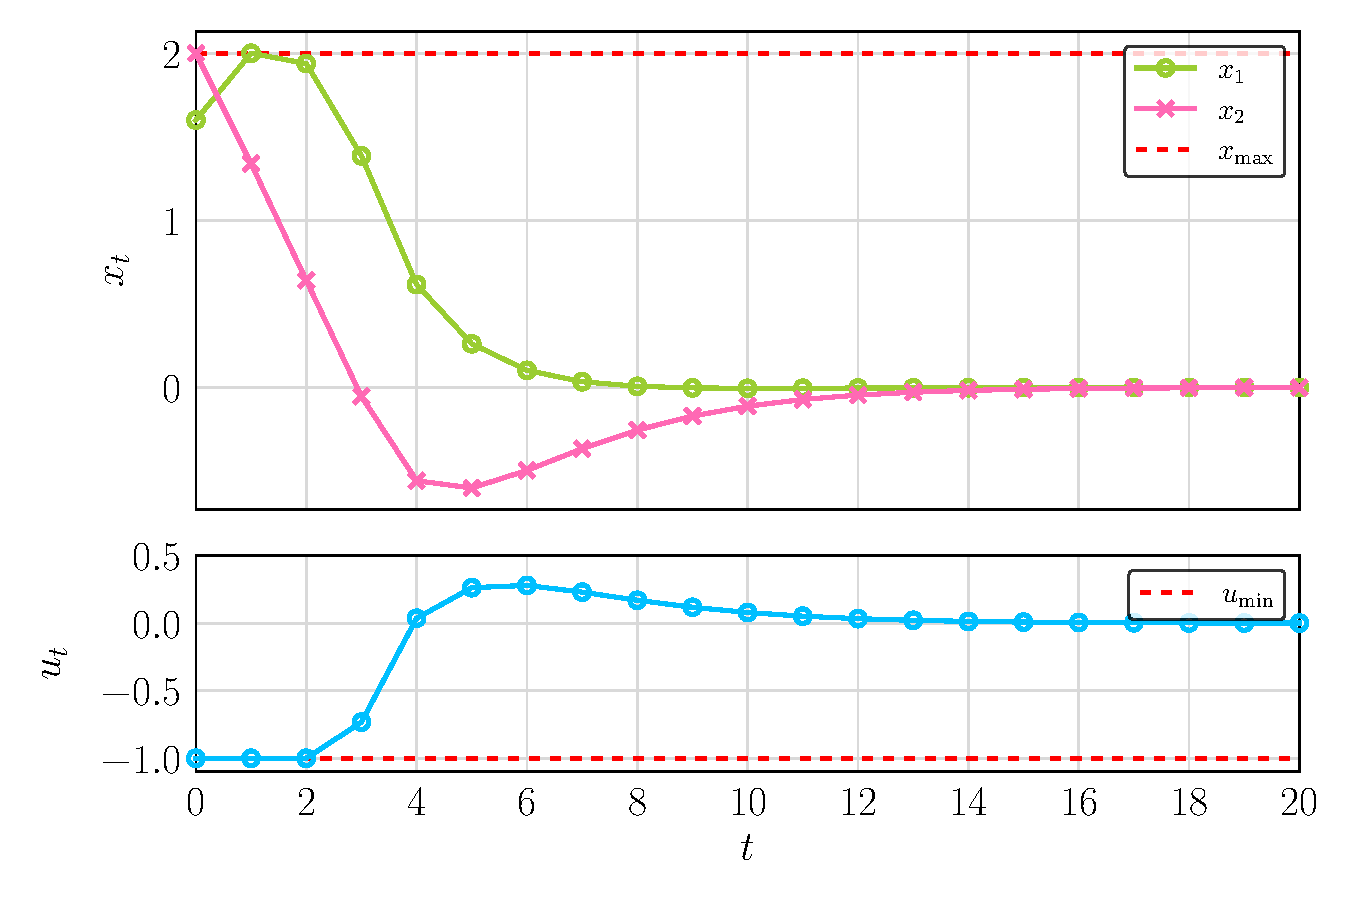
\includegraphics[width=0.7\linewidth]{figures/q3_i_xt_ut.pdf}
%     \caption{In the above plot we see the states changing of the MPC-
%     controlled system with $N = 10$, and in the below plot we see the control actions changing of the MPC-
%     controlled system with $N = 10$, starting from the extreme point $\begin{bsmallmatrix}1.6\\2\end{bsmallmatrix}$. 
%     We can observe that $x_t$ is steered in $20$ steps to $X_0(\{0\})$.}
%     \label{fig:q3_i_xt_ut}
% \end{figure}
% \begin{figure}[H]
%     \centering
%     \vspace{-0.35cm}
%     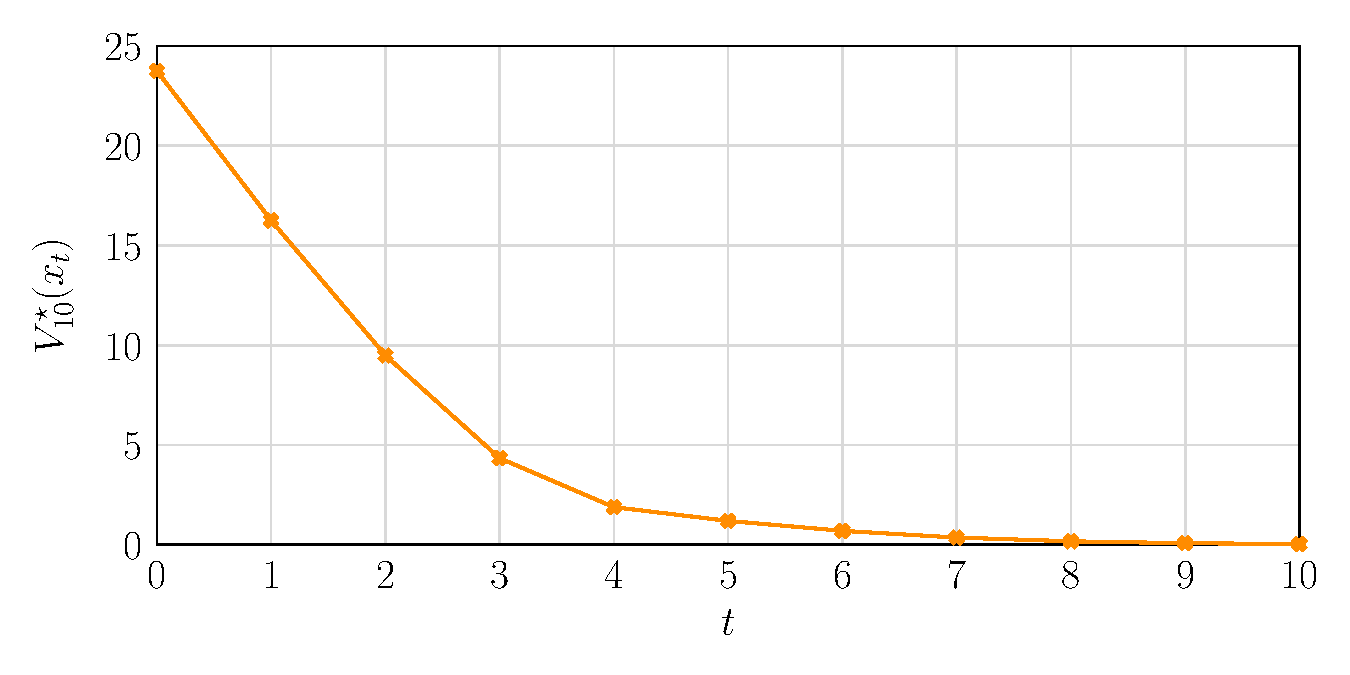
\includegraphics[width=0.7\linewidth]{figures/q3_i_cost.pdf}
%     \caption{The ``energy'' of the system as measured by the Lyapunov function $V^{\star}_{10}$ for the MPC-controlled system with $N = 10$.}
%     \label{fig:q3_i_cost}
% \end{figure}
\begin{figure}[H] %插入图片
    \raggedright
    \begin{subfigure}{0.45\linewidth}
        \begin{tikzpicture}                 % 绘图开始
            \begin{axis}[                   % 添加坐标
                % xlabel=$t$,
                ylabel=$x_t$,
                xmin=0, xmax=20,
                ymin=-1, ymax=2.2,
                xtick distance=2,
                ytick distance=1,
                xticklabels=\empty,
                grid=major,
                width=13cm,
                height=6cm,
                ]
                \addplot [line width=1pt,color=yellow-green,mark=o] % x_1
                coordinates                         % 声明是在迪卡尔坐标系中的数据
                {                                   % 输入数据
                    (0, 1.600000)
                    (1, 2.000000)
                    (2, 1.938000)
                    (3, 1.386000)
                    (4, 0.615531)
                    (5, 0.260837)
                    (6, 0.101978)
                    (7, 0.033747)
                    (8, 0.006417)
                    (9, -0.003134)
                    (10, -0.005414)
                    (11, -0.005042)
                    (12, -0.003937)
                    (13, -0.002829)
                    (14, -0.001936)
                    (15, -0.001285)
                    (16, -0.000835)
                    (17, -0.000534)
                    (18, -0.000338)
                    (19, -0.000212)
                    (20, -0.000132)
                    (21, -0.000082)
                    (22, -0.000051)
                    (23, -0.000031)
                    (24, -0.000019)
                    (25, -0.000012)
                    (26, -0.000007)
                    (27, -0.000004)
                    (28, -0.000002)
                    (29, -0.000001)
                    (30, -0.000001)
                    (31, -0.000000)
                    (32, -0.000000)
                    (33, -0.000000)
                    (34, -0.000000)
                    (35, -0.000000)
                    (36, -0.000000)
                    (37, -0.000000)
                    (38, -0.000000)
                    (39, -0.000000)
                    (40, -0.000000)
                };
                \addlegendentry{$x_{1}$}
                \addplot [line width=1pt,color=brinkpink,mark=x] % x_2
                coordinates                         % 声明是在迪卡尔坐标系中的数据
                {
                    (0, 2.000000)
                    (1, 1.340000)
                    (2, 0.640000)
                    (3, -0.053800)
                    (4, -0.558804)
                    (5, -0.602123)
                    (6, -0.496893)
                    (7, -0.367294)
                    (8, -0.255780)
                    (9, -0.171674)
                    (10, -0.112415)
                    (11, -0.072342)
                    (12, -0.045966)
                    (13, -0.028930)
                    (14, -0.018075)
                    (15, -0.011230)
                    (16, -0.006946)
                    (17, -0.004281)
                    (18, -0.002631)
                    (19, -0.001613)
                    (20, -0.000988)
                    (21, -0.000604)
                    (22, -0.000369)
                    (23, -0.000225)
                    (24, -0.000137)
                    (25, -0.000083)
                    (26, -0.000051)
                    (27, -0.000031)
                    (28, -0.000019)
                    (29, -0.000011)
                    (30, -0.000007)
                    (31, -0.000004)
                    (32, -0.000003)
                    (33, -0.000002)
                    (34, -0.000001)
                    (35, -0.000001)
                    (36, -0.000000)
                    (37, -0.000000)
                    (38, -0.000000)
                    (39, -0.000000)
                    (40, -0.000000)
                };
                \addlegendentry{$x_{2}$}
                \addplot [dashed,line width=1pt,color=red] % x_max
                coordinates                         % 声明是在迪卡尔坐标系中的数据
                {
                    (0, 2)
                    (1, 2)
                    (2, 2)
                    (3, 2)
                    (4, 2)
                    (5, 2)
                    (6, 2)
                    (7, 2)
                    (8, 2)
                    (9, 2)
                    (10, 2)
                    (11, 2)
                    (12, 2)
                    (13, 2)
                    (14, 2)
                    (15, 2)
                    (16, 2)
                    (17, 2)
                    (18, 2)
                    (19, 2)
                    (20, 2)
                    (21, 2)
                    (22, 2)
                    (23, 2)
                    (24, 2)
                    (25, 2)
                    (26, 2)
                    (27, 2)
                    (28, 2)
                    (29, 2)                   
                };
                \addlegendentry{$x_{\max}$}
            \end{axis}                         % 结束坐标
        \end{tikzpicture}                      % 绘图结束
    \end{subfigure}
    \\[\baselineskip]
    \vspace{-20pt}
    \begin{subfigure}{0.45\linewidth}
        \begin{tikzpicture}                 % 绘图开始
            \begin{axis}[                   % 添加坐标
                xlabel=$t$,
                ylabel=$u_t$,
                xmin=0, xmax=20,
                ymin=-1.1, ymax=0.5,
                xtick distance=2,
                ytick distance=0.5,
                grid=major,
                width=13cm,
                height=4cm,
                ]
                \addplot [line width=1pt,color=cornflowerblue,mark=o] % u_t
                coordinates                         % 声明是在迪卡尔坐标系中的数据
                {                                   % 输入数据
                    (0, -1.000000)
                    (1, -1.000000)
                    (2, -1.000000)
                    (3, -0.732809)
                    (4, 0.036468)
                    (5, 0.262628)
                    (6, 0.279594)
                    (7, 0.229776)
                    (8, 0.169496)
                    (9, 0.117891)
                    (10, 0.079063)
                    (11, 0.051744)
                    (12, 0.033285)
                    (13, 0.021143)
                    (14, 0.013304)
                    (15, 0.008311)
                    (16, 0.005163)
                    (17, 0.003193)
                    (18, 0.001968)
                    (19, 0.001209)
                    (20, 0.000741)
                    (21, 0.000454)
                    (22, 0.000278)
                    (23, 0.000169)
                    (24, 0.000103)
                    (25, 0.000063)
                    (26, 0.000038)
                    (27, 0.000023)
                    (28, 0.000014)
                    (29, 0.000009)
                    (30, 0.000005)
                    (31, 0.000003)
                    (32, 0.000002)
                    (33, 0.000001)
                    (34, 0.000001)
                    (35, 0.000000)
                    (36, 0.000000)
                    (37, 0.000000)
                    (38, 0.000000)
                    (39, 0.000000)
                };
                \addlegendentry{$u$}
                \addplot [dashed,line width=1pt,color=red]      % 调用绘图函数,并设置绘图的类型是折线图
                coordinates                         % 声明是在迪卡尔坐标系中的数据
                {                                   % 输入数据
                (0, -1)
                (1, -1)
                (2, -1)
                (3, -1)
                (4, -1)
                (5, -1)
                (6, -1)
                (7, -1)
                (8, -1)
                (9, -1)
                (10, -1)
                (11, -1)
                (12, -1)
                (13, -1)
                (14, -1)
                (15, -1)
                (16, -1)
                (17, -1)
                (18, -1)
                (19, -1)
                (20, -1)
                (21, -1)
                (22, -1)
                (23, -1)
                (24, -1)
                (25, -1)
                (26, -1)
                (27, -1)
                (28, -1)
                (29, -1)   
                };
                \addlegendentry{$u_{\min}$}
            \end{axis}                         % 结束坐标
        \end{tikzpicture}                      % 绘图结束
    \end{subfigure}
    \captionsetup{justification   = raggedright,
              singlelinecheck = false}
    \caption{In the above plot we see the states changing of the MPC-
        controlled system with $N = 10$, and in the below plot we see the control actions changing of the MPC-
        controlled system with $N = 10$, starting from the extreme point $\begin{bsmallmatrix}1.6\\2\end{bsmallmatrix}$. 
        We can observe that $x_t$ is steered in $20$ steps to $X_0(\{0\})$.}
    \label{fig:q3_i_xt_ut}
\end{figure}
\begin{figure}[H] %插入图片
    \raggedright
    \begin{tikzpicture}                 % 绘图开始
        \begin{axis}[                   % 添加坐标
            xlabel=$t$,
            ylabel=$V_{10}^{\star}(x_t)$,
            xmin=0, xmax=10,
            ymin=0, ymax=25,
            xtick distance=1,
            ytick distance=5,
            grid=major,
            width=13cm,
            height=6.5cm,
            ]
            \addplot [line width=1pt,color=orange,mark=x]      % 调用绘图函数,并设置绘图的类型是折线图
            coordinates                         % 声明是在迪卡尔坐标系中的数据
            {                                   % 输入数据
                (0, 23.751363)
                (1, 16.255833)
                (2, 9.490172)
                (3, 4.337820)
                (4, 1.882418)
                (5, 1.192190)
                (6, 0.693525)
                (7, 0.358401)
                (8, 0.169697)
                (9, 0.075556)
                (10, 0.032196)
            };
        \end{axis}                         % 结束坐标
    \end{tikzpicture}                      % 绘图结束
    \captionsetup{justification   = raggedright,
              singlelinecheck = false}
    \caption{The ``energy'' of the system as measured by the Lyapunov function $V^{\star}_{10}$ for the MPC-controlled system with $N = 10$.}
    \label{fig:q3_i_cost}
\end{figure}
\noindent(ii) Design an MPC by following the procedure outlined in Handout 10, Sections 10.2 and 10.3. Use
a prediction horizon $N=10$ and compute the set of feasible states, $X_N$. Simulate the MPC-controlled
system starting from the extreme points of $X_N$.
\\ \\
\textbf{Answer:} 
The Python code: \href{https://github.com/Gczmy/ELE8088/blob/main/Coursework1/Python_code/3_ii.py}{Question 1.3 (ii)}.
\\
The MPC-controlled dynamical system with $N=10$, using one of the extreme points of $X_N$ as the initial state, $x_0=\begin{bsmallmatrix}\ \ 2\\-2\end{bsmallmatrix}$.
\\
MPC controller:
\begin{subequations}
    \begin{align}
        \mathbb{P}_N(x){}:{}
        \operatorname*{Minimise}_{\substack{u_0,u_1,\ldots,u_{N-1}\\ x_0,x_1,\ldots,x_N}}&\sum_{t=0}^{N-1} (\left\lVert x_t\right\rVert ^2_2+u_t^2),
        \\
        \text{subject to: }& x_{t+1} = 
        \begin{bsmallmatrix}
            1&0.7\\
            -0.1&1
        \end{bsmallmatrix}x_t + 
        \begin{bsmallmatrix}
            1\\
            0.5
        \end{bsmallmatrix}u_t, t\in\N_{[0,N-1]},
        \\
        &\begin{bsmallmatrix}
            -2\\
            -2
        \end{bsmallmatrix} 
        \leq x_t \leq 
        \begin{bsmallmatrix}
            2\\
            2
        \end{bsmallmatrix}, t\in\N_{[1,N]},
        \\
        &-1 \leq u_t \leq 1, t\in\N_{[0,N-1]},
        \\
        & x_0 = \begin{bsmallmatrix}\ \ 2\\-2\end{bsmallmatrix}.
    \end{align}
\end{subequations}
The set of feasible states is shown in Figure \ref{fig:q3_ii_Xx} below.
% \begin{figure}[H]
%     \centering
%     \vspace{-0.35cm}
%     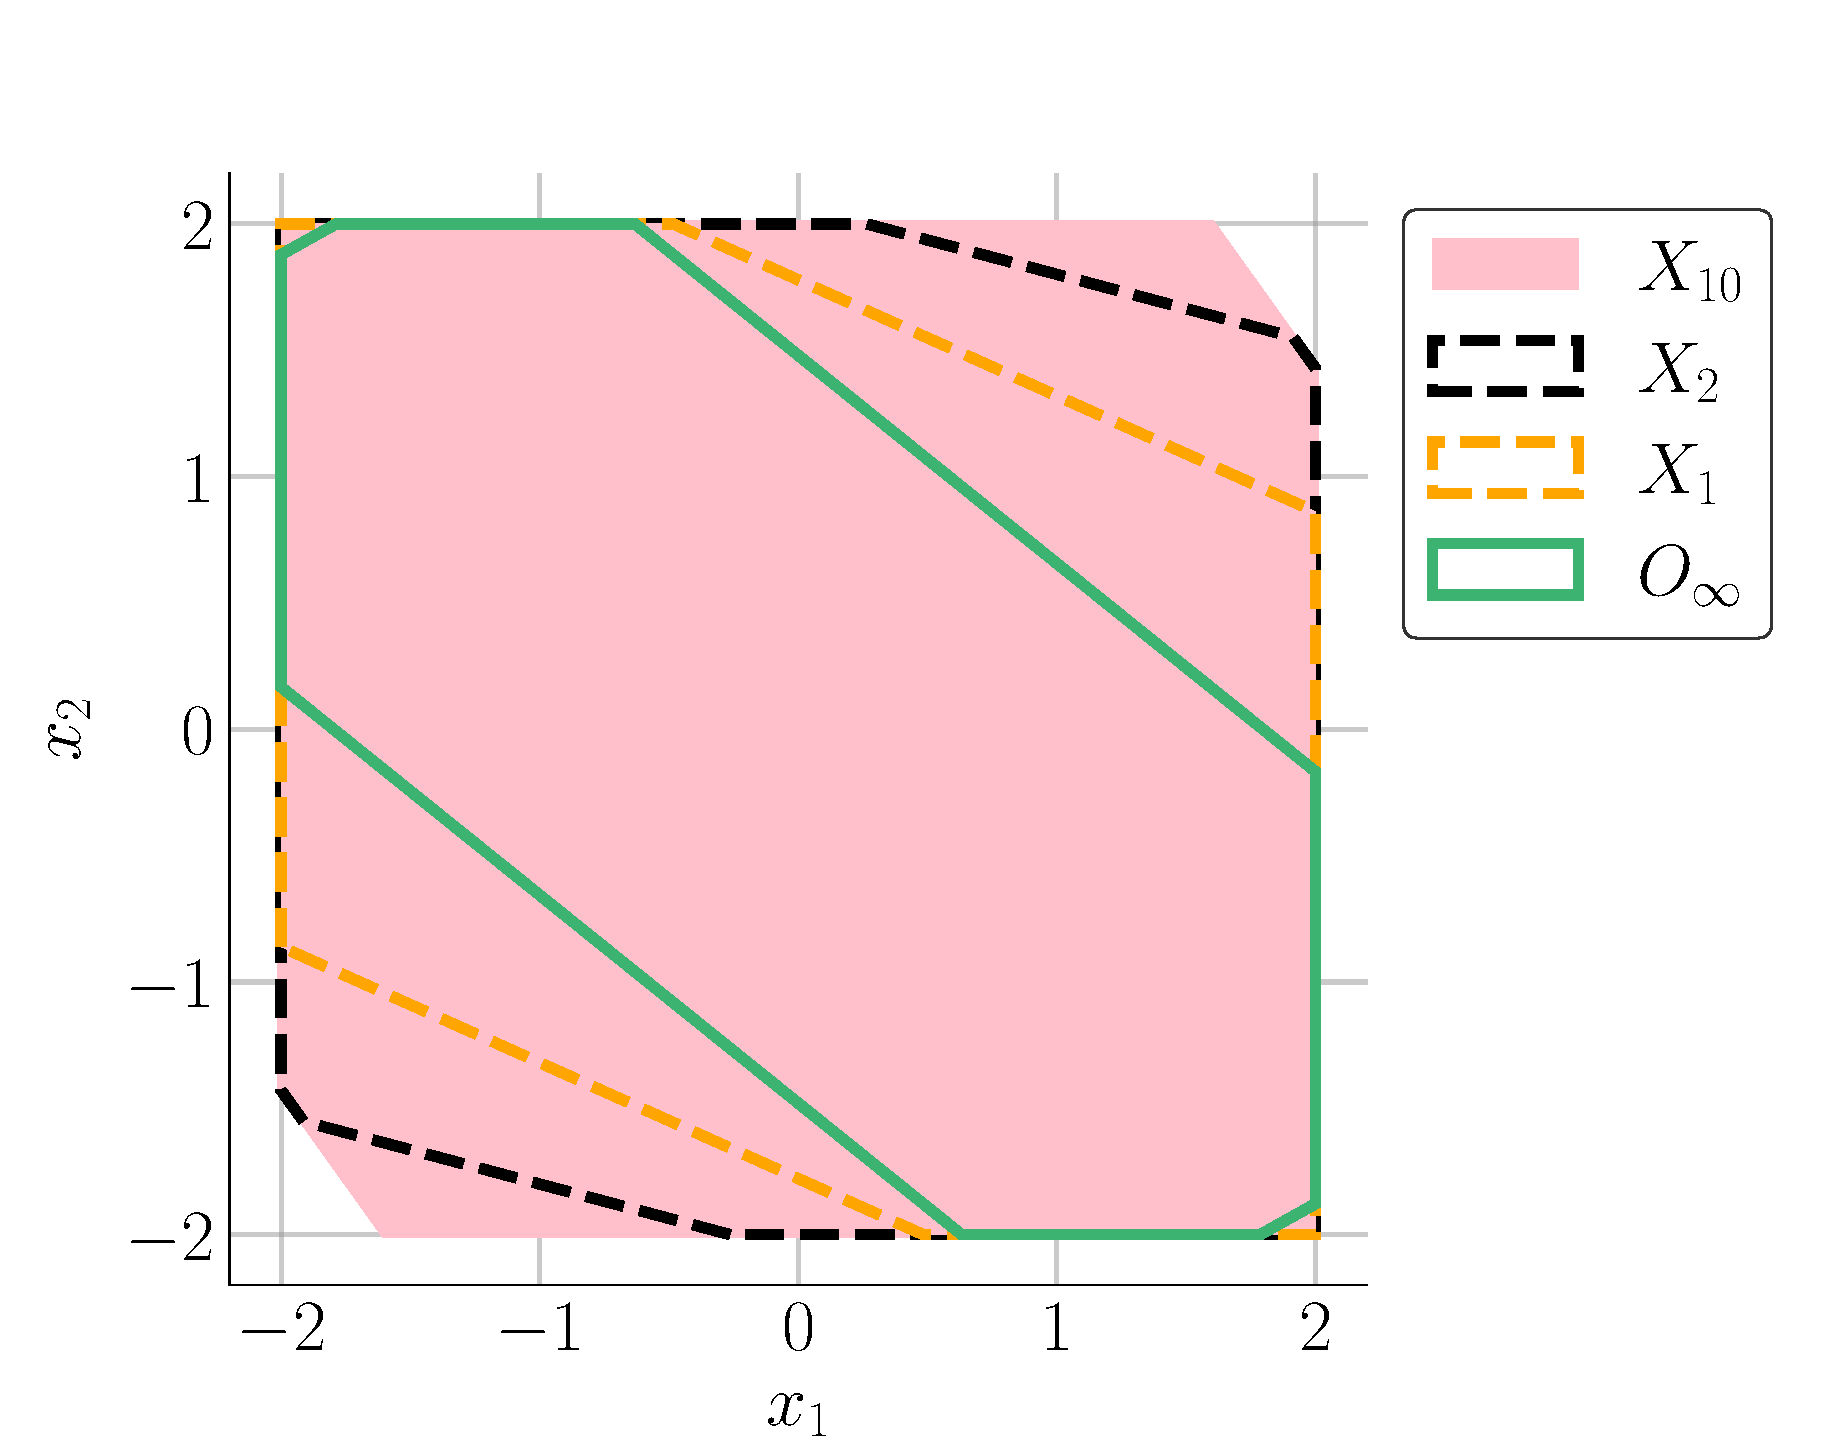
\includegraphics[width=0.45\linewidth]{figures/q3_ii_X.pdf}
%     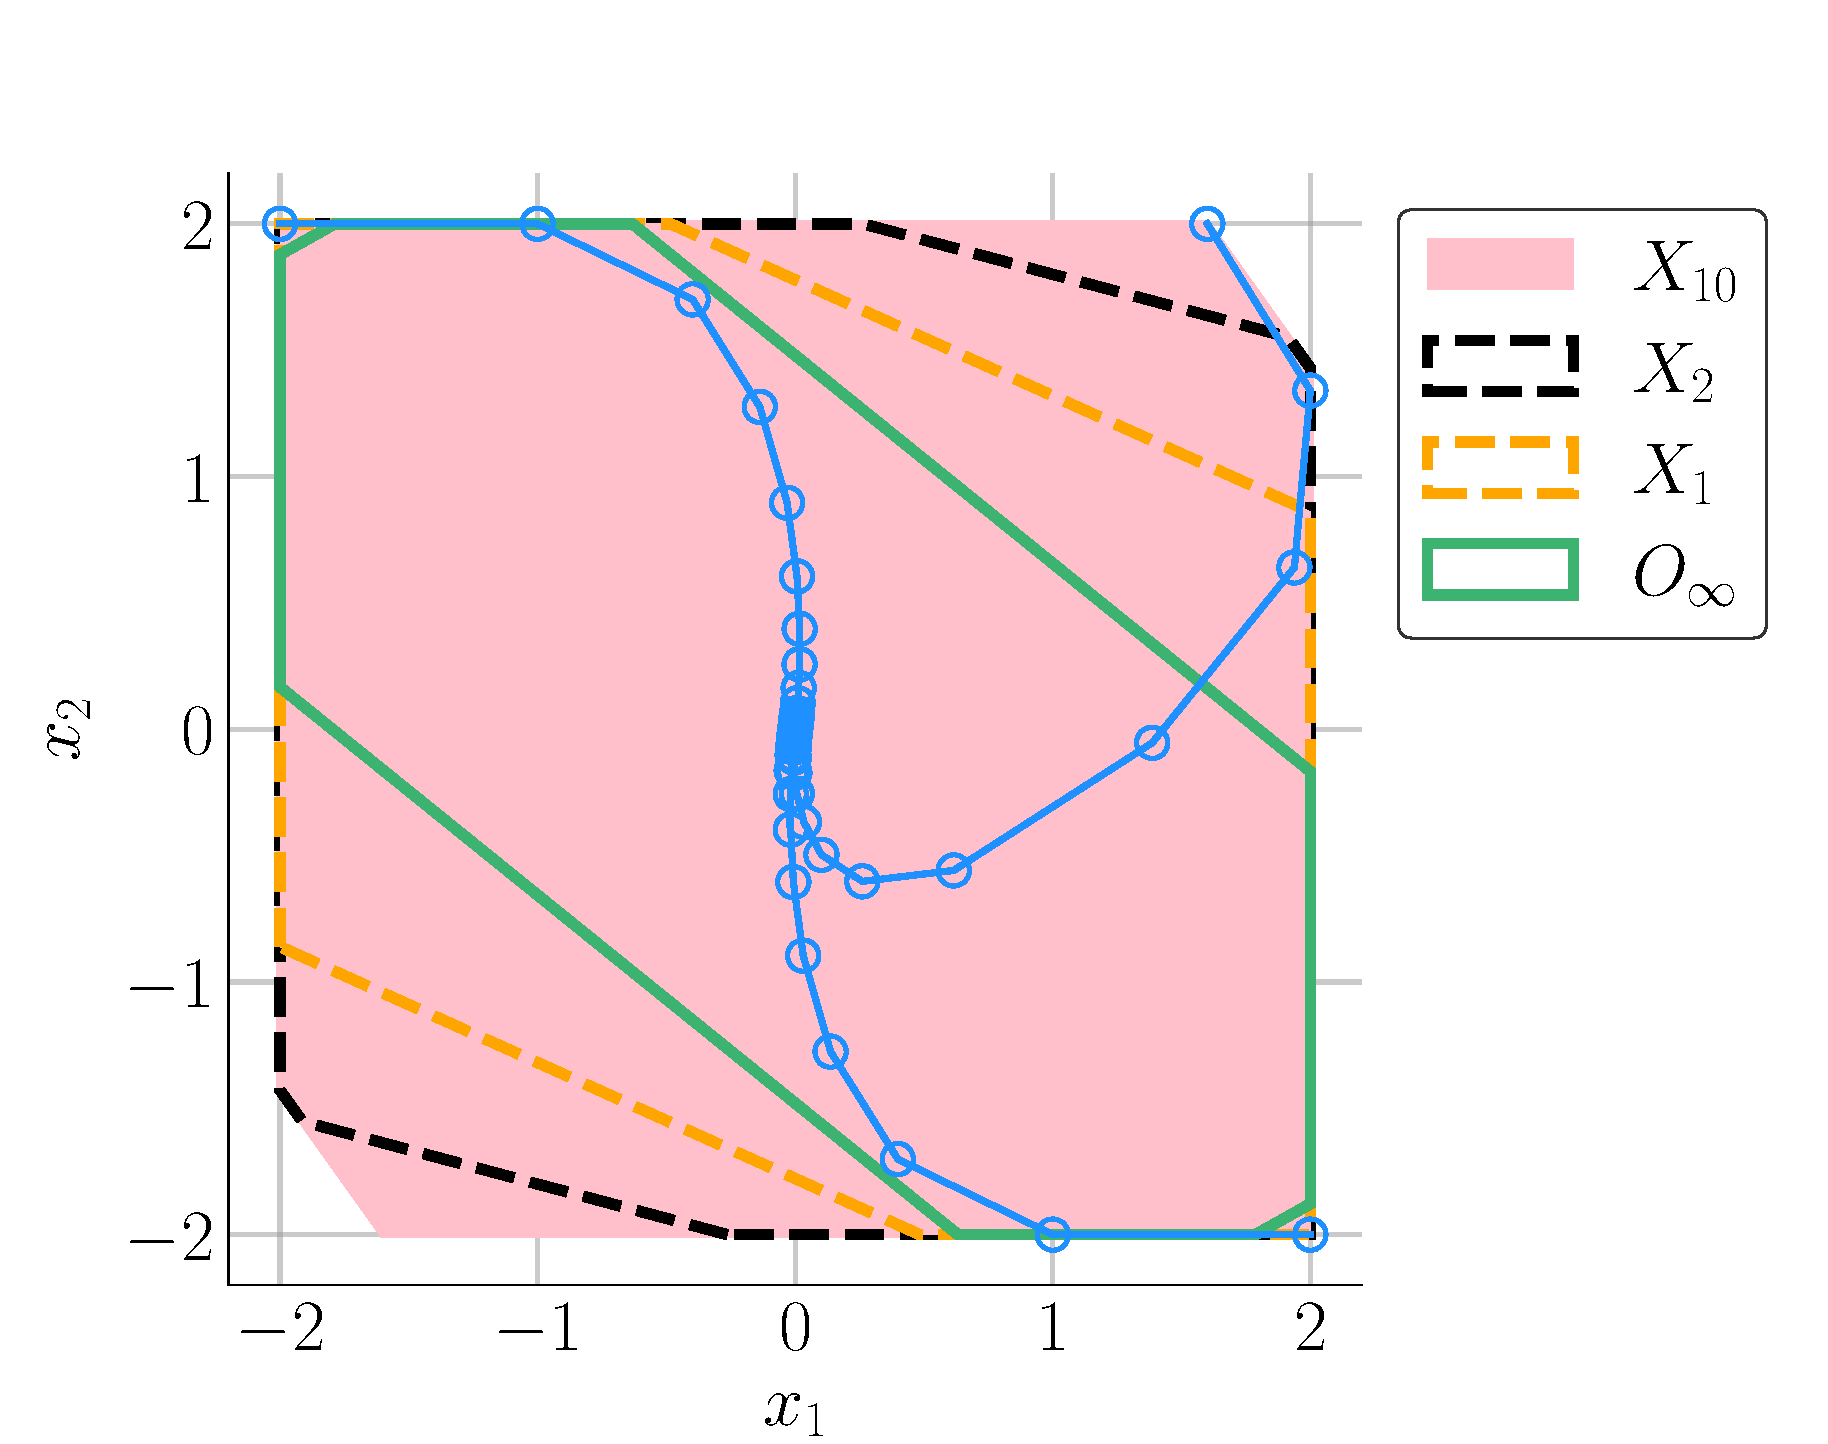
\includegraphics[width=0.45\linewidth]{figures/q3_ii_X_x.pdf}
    % \caption{We denote by $X_t(X_f)$ the set of states that can be steered in no more than $t$
    % steps to $X_f$. Observe that $Xt(O_{\infty})\subseteq Xt'(O_{\infty})$ for $t < t'$. In
    % other words, the larger the terminal set or the larger the prediction horizon is, the larger
    % the set of feasible states will be. In the right plot we see three trajectories of the
    % MPC-controlled system with $N = 10$, starting from three extreme points of $X_{10}(O_\infty)$. The extreme points are $\begin{bsmallmatrix}-2\\2\end{bsmallmatrix}, \begin{bsmallmatrix}1.6\\2\end{bsmallmatrix}, \begin{bsmallmatrix}2\\-2\end{bsmallmatrix}$. The set
    % $O_{\infty}$ is shown in all plots with green colour.
    % \label{fig:q3_ii_Xx}}
% \end{figure}
\begin{figure}[H] %插入图片
    \raggedright
    \begin{tikzpicture}                 % 绘图开始
        \begin{axis}[                   % 添加坐标
            axis x line*=bottom,
            axis y line*=left,
            xlabel=$x_1$,
            ylabel=$x_2$,
            xmin=-2.2, xmax=2.2,
            ymin=-2.2, ymax=2.2,
            xtick distance=1,
            ytick distance=1,
            grid=both,
            width=6.5cm,
            height=6.5cm,
            legend style={area legend,legend pos=outer north east},
            ]
            \addplot [pink,fill=pink]      % X_10
            coordinates                         % 声明是在迪卡尔坐标系中的数据
            {                                   % 输入数据
                (-1.6,     -2)
                (2,      -2)
                (2,       1.42857)
                (1.6,      2)
                (-2,       2)
                (-2,      -1.42857)
                (-1.6,     -2)
            };
            \addplot [dashed,line width=1.5pt,color=black]      % X_2
            coordinates                         % 声明是在迪卡尔坐标系中的数据
            {                                   % 输入数据
                (-1.91378,-1.55174)
                (-0.26359, -2 )    
                (2,      -2)     
                (2,       1.42857)
                (1.91378,  1.55174)
                (0.26359,  2  )   
                (-2,       2   )  
                (-2,      -1.42857)
                (-1.91378,-1.55174)
            };
            \addplot [dashed,line width=1.5pt,color=orange]      % X_1
            coordinates                         % 声明是在迪卡尔坐标系中的数据
            {                                   % 输入数据
                (0.48342, -2    ) 
                (2,      -2   )  
                (2,       0.86036)
                (-0.48342,  2)     
                (-2,       2)     
                (-2,      -0.86036)
                (0.48342, -2    )
            };
                \definecolor{mediumseagreen}{rgb}{0.24, 0.7, 0.44}
            \addplot [line width=1.5pt,color=mediumseagreen]      % O_{\infty}
            coordinates                         % 声明是在迪卡尔坐标系中的数据
            {                                   % 输入数据
                (0.63195 ,-2   )  
                (1.78679 ,-2  )   
                (2    ,  -1.8782 )
                (2  ,    -0.16714)
                (-0.63195 , 2  )   
                (-1.78679 , 2 )    
                (-2     ,  1.8782 )
                (-2    ,   0.16714)
                (0.63195 ,-2   )
            };
            \legend{$X_{10}$,$X_{2}$,$X_{1}$,$O_{\infty}$}
        \end{axis}                         % 结束坐标
    \end{tikzpicture}                      % 绘图结束
    \hspace{-25pt}
    \begin{tikzpicture}                 % 绘图开始
        \begin{axis}[                   % 添加坐标
            axis x line*=bottom,
            axis y line*=left,
            xlabel=$x_1$,
            ylabel=$x_2$,
            xmin=-2.2, xmax=2.2,
            ymin=-2.2, ymax=2.2,
            xtick distance=1,
            ytick distance=1,
            grid=both,
            width=6.5cm,
            height=6.5cm,
            area legend,
            legend style={legend pos=outer north east},
            ]
            \addplot [pink,fill=pink]      % X_10
            coordinates                         % 声明是在迪卡尔坐标系中的数据
            {                                   % 输入数据
                (-1.6,     -2)
                (2,      -2)
                (2,       1.42857)
                (1.6,      2)
                (-2,       2)
                (-2,      -1.42857)
                (-1.6,     -2)
            };
            \addplot [dashed,line width=1.5pt,color=black]      % X_2
            coordinates                         % 声明是在迪卡尔坐标系中的数据
            {                                   % 输入数据
                (-1.91378,-1.55174)
                (-0.26359, -2 )    
                (2,      -2)     
                (2,       1.42857)
                (1.91378,  1.55174)
                (0.26359,  2  )   
                (-2,       2   )  
                (-2,      -1.42857)
                (-1.91378,-1.55174)
            };
            \addplot [dashed,line width=1.5pt,color=orange]      % X_1
            coordinates                         % 声明是在迪卡尔坐标系中的数据
            {                                   % 输入数据
                (0.48342, -2    ) 
                (2,      -2   )  
                (2,       0.86036)
                (-0.48342,  2)     
                (-2,       2)     
                (-2,      -0.86036)
                (0.48342, -2    )
            };
                \definecolor{mediumseagreen}{rgb}{0.24, 0.7, 0.44}
            \addplot [line width=1.5pt,color=mediumseagreen]      % O_{\infty}
            coordinates                         % 声明是在迪卡尔坐标系中的数据
            {                                   % 输入数据
                (0.63195 ,-2   )  
                (1.78679 ,-2  )   
                (2    ,  -1.8782 )
                (2  ,    -0.16714)
                (-0.63195 , 2  )   
                (-1.78679 , 2 )    
                (-2     ,  1.8782 )
                (-2    ,   0.16714)
                (0.63195 ,-2   )
            };	\definecolor{dodgerblue}{rgb}{0.12, 0.56, 1.0}
            \addplot [line width=0.8pt,color=dodgerblue,mark=o,line legend]      % MPC
            coordinates                         % 声明是在迪卡尔坐标系中的数据
            {
                (2.000000, -2.000000)
                (1.000000, -2.000000)
                (0.398187, -1.700907)
                (0.137372, -1.275815)
                (0.031260, -0.896073)
                (-0.007071, -0.604739)
                (-0.017307, -0.397491)
                (-0.017009, -0.256490)
                (-0.013575, -0.163301)
                (-0.009865, -0.102933)
                (-0.006800, -0.064387)
                (-0.004534, -0.040039)
                (-0.002955, -0.024782)
                (-0.001895, -0.015283)
                (-0.001201, -0.009397)
                (-0.000754, -0.005765)
                (-0.000470, -0.003530)
                (-0.000292, -0.002158)
                (-0.000180, -0.001318)
                (-0.000111, -0.000804)
                (-0.000068, -0.000490)
                (-0.000042, -0.000299)
                (-0.000026, -0.000182)
                (-0.000016, -0.000111)
                (-0.000009, -0.000067)
                (-0.000006, -0.000041)
                (-0.000003, -0.000025)
                (-0.000002, -0.000015)
                (-0.000001, -0.000009)
                (-0.000001, -0.000006)
                (-0.000000, -0.000003)
                (-0.000000, -0.000002)
                (-0.000000, -0.000001)
                (-0.000000, -0.000001)
                (-0.000000, -0.000001)
                (-0.000000, -0.000000)
                (-0.000000, -0.000000)
                (-0.000000, -0.000000)
                (-0.000000, -0.000000)
                (-0.000000, -0.000000)
                (-0.000000, -0.000000)          
            };
            \addplot [line width=0.8pt,color=dodgerblue,mark=o]      % MPC
            coordinates                         % 声明是在迪卡尔坐标系中的数据
            {
                (1.600000, 2.000000)
                (2.000000, 1.340000)
                (1.938000, 0.640000)
                (1.386000, -0.053800)
                (0.615531, -0.558804)
                (0.260837, -0.602123)
                (0.101978, -0.496893)
                (0.033747, -0.367294)
                (0.006417, -0.255780)
                (-0.003134, -0.171674)
                (-0.005414, -0.112415)
                (-0.005042, -0.072342)
                (-0.003937, -0.045966)
                (-0.002829, -0.028930)
                (-0.001936, -0.018075)
                (-0.001285, -0.011230)
                (-0.000835, -0.006946)
                (-0.000534, -0.004281)
                (-0.000338, -0.002631)
                (-0.000212, -0.001613)
                (-0.000132, -0.000988)
                (-0.000082, -0.000604)
                (-0.000051, -0.000369)
                (-0.000031, -0.000225)
                (-0.000019, -0.000137)
                (-0.000012, -0.000083)
                (-0.000007, -0.000051)
                (-0.000004, -0.000031)
                (-0.000002, -0.000019)
                (-0.000001, -0.000011)
                (-0.000001, -0.000007)
                (-0.000000, -0.000004)
                (-0.000000, -0.000003)
                (-0.000000, -0.000002)
                (-0.000000, -0.000001)
                (-0.000000, -0.000001)
                (-0.000000, -0.000000)
            };
            \addplot [line width=0.8pt,color=dodgerblue,mark=o]      % MPC
            coordinates                         % 声明是在迪卡尔坐标系中的数据
            {
                (-2.000000, 2.000000)
                (-1.000000, 2.000000)
                (-0.398187, 1.700907)
                (-0.137372, 1.275815)
                (-0.031260, 0.896073)
                (0.007071, 0.604739)
                (0.017307, 0.397491)
                (0.017009, 0.256490)
                (0.013575, 0.163301)
                (0.009865, 0.102933)
                (0.006800, 0.064387)
                (0.004534, 0.040039)
                (0.002955, 0.024782)
                (0.001895, 0.015283)
                (0.001201, 0.009397)
                (0.000754, 0.005765)
                (0.000470, 0.003530)
                (0.000292, 0.002158)
                (0.000180, 0.001318)
                (0.000111, 0.000804)
                (0.000068, 0.000490)
                (0.000042, 0.000299)
                (0.000026, 0.000182)
                (0.000016, 0.000111)
                (0.000009, 0.000067)
                (0.000006, 0.000041)
                (0.000003, 0.000025)
                (0.000002, 0.000015)
                (0.000001, 0.000009)
                (0.000001, 0.000006)
                (0.000000, 0.000003)
                (0.000000, 0.000002)
                (0.000000, 0.000001)
                (0.000000, 0.000001)
                (0.000000, 0.000001)
                (0.000000, 0.000000)
            };
            \legend{$X_{10}$,$X_{2}$,$X_{1}$,$O_{\infty}$,MPC}
        \end{axis}                         % 结束坐标
    \end{tikzpicture}                      % 绘图结束
    \captionsetup{justification   = raggedright,
              singlelinecheck = false}
    \caption{We denote by $X_t(X_f)$ the set of states that can be steered in no more than $t$
    steps to $X_f$. Observe that $Xt(O_{\infty})\subseteq Xt'(O_{\infty})$ for $t < t'$. In
    other words, the larger the terminal set or the larger the prediction horizon is, the larger
    the set of feasible states will be. In the right plot we see three trajectories of the
    MPC-controlled system with $N = 10$, starting from three extreme points of $X_{10}(O_\infty)$. The extreme points are $\begin{bsmallmatrix}-2\\2\end{bsmallmatrix}, \begin{bsmallmatrix}1.6\\2\end{bsmallmatrix}, \begin{bsmallmatrix}2\\-2\end{bsmallmatrix}$. The set
    $O_{\infty}$ is shown in all plots with green colour.
    \label{fig:q3_ii_Xx}}
\end{figure}
The simulation of the MPC-controlled dynamical system is shown in Figure \ref{fig:q3_ii_xt_ut} and Figure \ref{fig:q3_ii_cost} below.
\begin{figure}[H] %插入图片
    \raggedright
    \begin{subfigure}{0.45\linewidth}
        \begin{tikzpicture}                 % 绘图开始
            \begin{axis}[                   % 添加坐标
                % xlabel=$t$,
                ylabel=$x_t$,
                xmin=0, xmax=20,
                ymin=-1, ymax=2.2,
                xtick distance=2,
                ytick distance=1,
                xticklabels=\empty,
                grid=major,
                width=13cm,
                height=6cm,
                ]
                \addplot [line width=1pt,color=yellow-green,mark=o] % x_1
                coordinates                         % 声明是在迪卡尔坐标系中的数据
                {                                   % 输入数据
                    (0, 1.600000)
                    (1, 2.000000)
                    (2, 1.938000)
                    (3, 1.386000)
                    (4, 0.615531)
                    (5, 0.260837)
                    (6, 0.101978)
                    (7, 0.033747)
                    (8, 0.006417)
                    (9, -0.003134)
                    (10, -0.005414)
                    (11, -0.005042)
                    (12, -0.003937)
                    (13, -0.002829)
                    (14, -0.001936)
                    (15, -0.001285)
                    (16, -0.000835)
                    (17, -0.000534)
                    (18, -0.000338)
                    (19, -0.000212)
                    (20, -0.000132)
                    (21, -0.000082)
                    (22, -0.000051)
                    (23, -0.000031)
                    (24, -0.000019)
                    (25, -0.000012)
                    (26, -0.000007)
                    (27, -0.000004)
                    (28, -0.000002)
                    (29, -0.000001)
                    (30, -0.000001)
                    (31, -0.000000)
                    (32, -0.000000)
                    (33, -0.000000)
                    (34, -0.000000)
                    (35, -0.000000)
                    (36, -0.000000)
                    (37, -0.000000)
                    (38, -0.000000)
                    (39, -0.000000)
                    (40, -0.000000)
                };
                \addlegendentry{$x_{1}$}
                \addplot [line width=1pt,color=brinkpink,mark=x] % x_2
                coordinates                         % 声明是在迪卡尔坐标系中的数据
                {
                    (0, 2.000000)
                    (1, 1.340000)
                    (2, 0.640000)
                    (3, -0.053800)
                    (4, -0.558804)
                    (5, -0.602123)
                    (6, -0.496893)
                    (7, -0.367294)
                    (8, -0.255780)
                    (9, -0.171674)
                    (10, -0.112415)
                    (11, -0.072342)
                    (12, -0.045966)
                    (13, -0.028930)
                    (14, -0.018075)
                    (15, -0.011230)
                    (16, -0.006946)
                    (17, -0.004281)
                    (18, -0.002631)
                    (19, -0.001613)
                    (20, -0.000988)
                    (21, -0.000604)
                    (22, -0.000369)
                    (23, -0.000225)
                    (24, -0.000137)
                    (25, -0.000083)
                    (26, -0.000051)
                    (27, -0.000031)
                    (28, -0.000019)
                    (29, -0.000011)
                    (30, -0.000007)
                    (31, -0.000004)
                    (32, -0.000003)
                    (33, -0.000002)
                    (34, -0.000001)
                    (35, -0.000001)
                    (36, -0.000000)
                    (37, -0.000000)
                    (38, -0.000000)
                    (39, -0.000000)
                    (40, -0.000000)                    
                };
                \addlegendentry{$x_{2}$}
                \addplot [dashed,line width=1pt,color=red] % x_max
                coordinates                         % 声明是在迪卡尔坐标系中的数据
                {
                    (0, 2)
                    (1, 2)
                    (2, 2)
                    (3, 2)
                    (4, 2)
                    (5, 2)
                    (6, 2)
                    (7, 2)
                    (8, 2)
                    (9, 2)
                    (10, 2)
                    (11, 2)
                    (12, 2)
                    (13, 2)
                    (14, 2)
                    (15, 2)
                    (16, 2)
                    (17, 2)
                    (18, 2)
                    (19, 2)
                    (20, 2)
                    (21, 2)
                    (22, 2)
                    (23, 2)
                    (24, 2)
                    (25, 2)
                    (26, 2)
                    (27, 2)
                    (28, 2)
                    (29, 2)                   
                };
                \addlegendentry{$x_{\max}$}
            \end{axis}                         % 结束坐标
        \end{tikzpicture}                      % 绘图结束
    \end{subfigure}
    \\[\baselineskip]
    \vspace{-20pt}
    \begin{subfigure}{0.45\linewidth}
        \begin{tikzpicture}                 % 绘图开始
            \begin{axis}[                   % 添加坐标
                xlabel=$t$,
                ylabel=$u_t$,
                xmin=0, xmax=20,
                ymin=-1.1, ymax=0.5,
                xtick distance=2,
                ytick distance=0.5,
                grid=major,
                width=13cm,
                height=4cm,
                ]
                \addplot [line width=1pt,color=cornflowerblue,mark=o] % u_t
                coordinates                         % 声明是在迪卡尔坐标系中的数据
                {                                   % 输入数据
                    (0, -1.000000)
                    (1, -1.000000)
                    (2, -1.000000)
                    (3, -0.732809)
                    (4, 0.036468)
                    (5, 0.262628)
                    (6, 0.279594)
                    (7, 0.229776)
                    (8, 0.169496)
                    (9, 0.117891)
                    (10, 0.079063)
                    (11, 0.051744)
                    (12, 0.033285)
                    (13, 0.021143)
                    (14, 0.013304)
                    (15, 0.008311)
                    (16, 0.005163)
                    (17, 0.003193)
                    (18, 0.001968)
                    (19, 0.001209)
                    (20, 0.000741)
                    (21, 0.000454)
                    (22, 0.000278)
                    (23, 0.000169)
                    (24, 0.000103)
                    (25, 0.000063)
                    (26, 0.000038)
                    (27, 0.000023)
                    (28, 0.000014)
                    (29, 0.000009)
                    (30, 0.000005)
                    (31, 0.000003)
                    (32, 0.000002)
                    (33, 0.000001)
                    (34, 0.000001)
                    (35, 0.000000)
                    (36, 0.000000)
                    (37, 0.000000)
                    (38, 0.000000)
                    (39, 0.000000) 
                };
                \addlegendentry{$u$}
                \addplot [dashed,line width=1pt,color=red]      % 调用绘图函数,并设置绘图的类型是折线图
                coordinates                         % 声明是在迪卡尔坐标系中的数据
                {                                   % 输入数据
                (0, -1)
                (1, -1)
                (2, -1)
                (3, -1)
                (4, -1)
                (5, -1)
                (6, -1)
                (7, -1)
                (8, -1)
                (9, -1)
                (10, -1)
                (11, -1)
                (12, -1)
                (13, -1)
                (14, -1)
                (15, -1)
                (16, -1)
                (17, -1)
                (18, -1)
                (19, -1)
                (20, -1)
                (21, -1)
                (22, -1)
                (23, -1)
                (24, -1)
                (25, -1)
                (26, -1)
                (27, -1)
                (28, -1)
                (29, -1)   
                };
                \addlegendentry{$u_{\min}$}
            \end{axis}                         % 结束坐标
        \end{tikzpicture}                      % 绘图结束
    \end{subfigure}
    \captionsetup{justification   = raggedright,
              singlelinecheck = false}
    \caption{In the above plot we see the states changing of the MPC-
        controlled system with $N = 10$, and in the below plot we see the control actions changing of the MPC-
        controlled system with $N = 10$, starting from the extreme point $\begin{bsmallmatrix}1.6\\2\end{bsmallmatrix}$. 
        We can observe that $x_t$ is steered in $20$ steps to $O_{\infty}$.}
    \label{fig:q3_ii_xt_ut}
\end{figure}
\begin{figure}[H] %插入图片
    \raggedright
    \begin{tikzpicture}                 % 绘图开始
        \begin{axis}[                   % 添加坐标
            xlabel=$t$,
            ylabel=$V_{10}^{\star}(x_t)$,
            xmin=0, xmax=10,
            ymin=0, ymax=25,
            xtick distance=1,
            ytick distance=5,
            grid=major,
            width=13cm,
            height=6.5cm,
            ]
            \addplot [line width=1pt,color=orange,mark=x]      % 调用绘图函数,并设置绘图的类型是折线图
            coordinates                         % 声明是在迪卡尔坐标系中的数据
            {                                   % 输入数据
                (0, 23.751363)
                (1, 16.255833)
                (2, 9.490172)
                (3, 4.337820)
                (4, 1.882418)
                (5, 1.192190)
                (6, 0.693525)
                (7, 0.358401)
                (8, 0.169697)
                (9, 0.075556)
                (10, 0.032196)
            };
        \end{axis}                         % 结束坐标
    \end{tikzpicture}                      % 绘图结束
    \captionsetup{justification   = raggedright,
              singlelinecheck = false}
    \caption{The ``energy'' of the system as measured by the Lyapunov function $V^{\star}_{10}$ for the MPC-controlled system with $N = 10$.}
    \label{fig:q3_ii_cost}
\end{figure}
\noindent(iii) Design an MPC controller using an ellipsoidal terminal set and prediction horizon $N=10$. Provide simulation results starting from different initial states.
\\ \\
\textbf{Answer:} 
The Python code: \href{https://github.com/Gczmy/ELE8088/blob/main/Coursework1/Python_code/3_iii.py}{Question 1.3 (iii)}.
\\
Using an ellipsoidal terminal set, let
\begin{equation}
    \alpha \leq \min_{i\in\N_{[1,s]}}\frac{b_i^2}{\|P^{-1/2}h_i\|_2^2}
\end{equation}
MPC controller:
\begin{subequations}
    \begin{align}
        \mathbb{P}_N(x){}:{}
        \operatorname*{Minimise}_{\substack{u_0,u_1,\ldots,u_{N-1}\\ x_0,x_1,\ldots,x_N}}&\sum_{t=0}^{N-1} (\left\lVert x_t\right\rVert ^2_2+u_t^2) + \tfrac{1}{2}x_N^{\tran}P x_N,
        \\
        \text{subject to: }& x_{t+1} = 
        \begin{bsmallmatrix}
            1&0.7\\
            -0.1&1
        \end{bsmallmatrix}x_t + 
        \begin{bsmallmatrix}
            1\\
            0.5
        \end{bsmallmatrix}u_t, t\in\N_{[0,N-1]},
        \\
        &x_N^{\tran} P x_N \leq \alpha,
        \\
        &\begin{bsmallmatrix}
            -2\\
            -2
        \end{bsmallmatrix} 
        \leq x_t \leq 
        \begin{bsmallmatrix}
            2\\
            2
        \end{bsmallmatrix}, t\in\N_{[1,N]},
        \\
        &-1 \leq u_t \leq 1, t\in\N_{[0,N-1]},
        \\
        & x_0 = x.
    \end{align}
\end{subequations}
The simulation of the MPC-controlled dynamical system is shown in Figure \ref{fig:q3_iii_xt_ut} and Figure \ref{fig:q3_iii_cost} below.
\begin{figure}[H] %插入图片
    \raggedright
    \begin{subfigure}{0.45\linewidth}
        \begin{tikzpicture}                 % 绘图开始
            \begin{axis}[                   % 添加坐标
                % xlabel=$t$,
                ylabel=$x_t$,
                xmin=0, xmax=20,
                ymin=-2.2, ymax=2.2,
                xtick distance=2,
                ytick distance=1,
                xticklabels=\empty,
                grid=major,
                width=13cm,
                height=6cm,
                ]
                \addplot [line width=1pt,color=yellow-green,mark=o] % x_1
                coordinates                         % 声明是在迪卡尔坐标系中的数据
                {                                   % 输入数据
                (0, -2.000000)
                (1, -1.000000)
                (2, -0.396205)
                (3, -0.135230)
                (4, -0.029524)
                (5, 0.008318)
                (6, 0.018145)
                (7, 0.017548)
                (8, 0.013911)
                (9, 0.010068)
                (10, 0.006921)
                (11, 0.004604)
                (12, 0.002995)
                (13, 0.001918)
                (14, 0.001213)
                (15, 0.000761)
                (16, 0.000474)
                (17, 0.000294)
                (18, 0.000181)
                (19, 0.000111)
                (20, 0.000068)
                (21, 0.000042)
                (22, 0.000026)
                (23, 0.000016)
                (24, 0.000009)
                (25, 0.000006)
                (26, 0.000003)
                (27, 0.000002)
                (28, 0.000001)
                (29, 0.000000)
                (30, 0.000000)
                };
                \addlegendentry{$x_{1}$}
                \addplot [line width=1pt,color=brinkpink,mark=x] % x_2
                coordinates                         % 声明是在迪卡尔坐标系中的数据
                {
                (0, 2.000000)
                (1, 2.000000)
                (2, 1.701897)
                (3, 1.276342)
                (4, 0.895998)
                (5, 0.604272)
                (6, 0.396858)
                (7, 0.255845)
                (8, 0.162726)
                (9, 0.102460)
                (10, 0.064018)
                (11, 0.039761)
                (12, 0.024580)
                (13, 0.015139)
                (14, 0.009296)
                (15, 0.005695)
                (16, 0.003482)
                (17, 0.002126)
                (18, 0.001296)
                (19, 0.000790)
                (20, 0.000481)
                (21, 0.000292)
                (22, 0.000178)
                (23, 0.000108)
                (24, 0.000066)
                (25, 0.000040)
                (26, 0.000024)
                (27, 0.000015)
                (28, 0.000009)
                (29, 0.000005)
                (30, 0.000003)
                };
                \addlegendentry{$x_{2}$}
                \addplot [dashed,line width=1pt,color=red] % x_min
                coordinates                         % 声明是在迪卡尔坐标系中的数据
                {
                    (0, -2)
                    (1, -2)
                    (2, -2)
                    (3, -2)
                    (4, -2)
                    (5, -2)
                    (6, -2)
                    (7, -2)
                    (8, -2)
                    (9, -2)
                    (10, -2)
                    (11, -2)
                    (12, -2)
                    (13, -2)
                    (14, -2)
                    (15, -2)
                    (16, -2)
                    (17, -2)
                    (18, -2)
                    (19, -2)
                    (20, -2)
                    (21, -2)
                    (22, -2)
                    (23, -2)
                    (24, -2)
                    (25, -2)
                    (26, -2)
                    (27, -2)
                    (28, -2)
                    (29, -2)                    
                };
                \addlegendentry{$x_{\min}$}
                \addplot [dashed,line width=1pt,color=red] % x_max
                coordinates                         % 声明是在迪卡尔坐标系中的数据
                {
                    (0, 2)
                    (1, 2)
                    (2, 2)
                    (3, 2)
                    (4, 2)
                    (5, 2)
                    (6, 2)
                    (7, 2)
                    (8, 2)
                    (9, 2)
                    (10, 2)
                    (11, 2)
                    (12, 2)
                    (13, 2)
                    (14, 2)
                    (15, 2)
                    (16, 2)
                    (17, 2)
                    (18, 2)
                    (19, 2)
                    (20, 2)
                    (21, 2)
                    (22, 2)
                    (23, 2)
                    (24, 2)
                    (25, 2)
                    (26, 2)
                    (27, 2)
                    (28, 2)
                    (29, 2)                   
                };
                \addlegendentry{$x_{\max}$}
            \end{axis}                         % 结束坐标
        \end{tikzpicture}                      % 绘图结束
    \end{subfigure}
    \\[\baselineskip]
    \vspace{-20pt}
    \begin{subfigure}{0.45\linewidth}
        \begin{tikzpicture}                 % 绘图开始
            \begin{axis}[                   % 添加坐标
                xlabel=$t$,
                ylabel=$u_t$,
                xmin=0, xmax=20,
                ymin=-1.05, ymax=0.05,
                xtick distance=2,
                ytick distance=0.5,
                grid=major,
                width=13cm,
                height=4cm,
                ]
                \addplot [line width=1pt,color=cornflowerblue,mark=o]      % 调用绘图函数,并设置绘图的类型是折线图
                coordinates                         % 声明是在迪卡尔坐标系中的数据
                {                                   % 输入数据
                (0, -0.400000)
                (1, -0.796205)
                (2, -0.930352)
                (3, -0.787733)
                (4, -0.589356)
                (5, -0.413164)
                (6, -0.278398)
                (7, -0.182729)
                (8, -0.117750)
                (9, -0.074869)
                (10, -0.047130)
                (11, -0.029442)
                (12, -0.018284)
                (13, -0.011302)
                (14, -0.006960)
                (15, -0.004274)
                (16, -0.002618)
                (17, -0.001601)
                (18, -0.000977)
                (19, -0.000596)
                (20, -0.000363)   
                };
                \addlegendentry{$u$}
                \addplot [dashed,line width=1pt,color=red]      % 调用绘图函数,并设置绘图的类型是折线图
                coordinates                         % 声明是在迪卡尔坐标系中的数据
                {                                   % 输入数据
                (0, -1)
                (1, -1)
                (2, -1)
                (3, -1)
                (4, -1)
                (5, -1)
                (6, -1)
                (7, -1)
                (8, -1)
                (9, -1)
                (10, -1)
                (11, -1)
                (12, -1)
                (13, -1)
                (14, -1)
                (15, -1)
                (16, -1)
                (17, -1)
                (18, -1)
                (19, -1)
                (20, -1)
                (21, -1)
                (22, -1)
                (23, -1)
                (24, -1)
                (25, -1)
                (26, -1)
                (27, -1)
                (28, -1)
                (29, -1)   
                };
                \addlegendentry{$u_{\min}$}
            \end{axis}                         % 结束坐标
        \end{tikzpicture}                      % 绘图结束
    \end{subfigure}
    \captionsetup{justification   = raggedright,
              singlelinecheck = false}
    \caption{In the above plot we see the states changing of the MPC-
    controlled system with $N = 10$, and in the below plot we see the control actions changing of the MPC-
    controlled system with $N = 10$, starting from the extreme point $\begin{bsmallmatrix}-2\\2\end{bsmallmatrix}$. 
    We can observe that $x_t$ is steered in $20$ steps to $X_f$.}
    \label{fig:q3_iii_xt_ut}
\end{figure}
\begin{figure}[H] %插入图片
    \raggedright
    \begin{tikzpicture}                 % 绘图开始
        \begin{axis}[                   % 添加坐标
            xlabel=$t$,
            ylabel=$V_{10}^{\star}(x_t)$,
            xmin=0, xmax=10,
            ymin=0, ymax=25,
            xtick distance=1,
            ytick distance=5,
            grid=major,
            width=13cm,
            height=6.5cm,
            ]
            \addplot [line width=1pt,color=orange,mark=x]      % 调用绘图函数,并设置绘图的类型是折线图
            coordinates                         % 声明是在迪卡尔坐标系中的数据
            {                                   % 输入数据
                (0, 22.053813)
                (1, 13.903255)
                (2, 8.273036)
                (3, 4.355495)
                (4, 2.088193)
                (5, 0.937381)
                (6, 0.401543)
                (7, 0.166242)
                (8, 0.067099)
                (9, 0.026565)
                (10, 0.010362)    
            };
        \end{axis}                         % 结束坐标
    \end{tikzpicture}                      % 绘图结束
    \captionsetup{justification   = raggedright,
              singlelinecheck = false}
    \caption{The ``energy'' of the system as measured by the Lyapunov function $V^{\star}_{10}$ for the MPC-controlled system with $N = 10$.}
    \label{fig:q3_iii_cost}
\end{figure}
Now consider the nonlinear dynamical system\footnote[2]{We denote the two coordinates of $x_t\in\R^2$ by $x_{t,1}$ and $x_{t,2}$}.
\begin{equation}
    x_{t+1}=
    \begin{bmatrix}
        1&0.7\\
        -0.1&1
    \end{bmatrix}
    x_t+
    \begin{bmatrix}
        1\\
        0.5
    \end{bmatrix}
    u_t+
    \frac{1}{20}
    \begin{bmatrix}
        x_t^{\tran}x_t\\
        \sin^2(x_{t,1})
    \end{bmatrix},
\end{equation}
which is subject to the constraints given in \eqref{eq:q2_constraints}.
\\ \\
(iv) Design a nonlinear model predictive controller using the methodology of Section 10.6 in Handout 10: determine the terminal cost function and the terminal set of constraints.
\\ \\
\textbf{Answer:} 
The Python code: \href{https://github.com/Gczmy/ELE8088/blob/main/Coursework1/Python_code/3_iv.py}{Question 1.3 (iv)}.
\\
Choose $\ell(x,u)=\tfrac{1}{2}(x^{\tran}Qx+u^{\tran}Ru)=\left\lVert x\right\rVert ^2_2+u^2$, hence $Q=\begin{bsmallmatrix}\sqrt{2}&0\\0&\sqrt{2}\end{bsmallmatrix},R=\sqrt{2}.$
Let $K$ be a stabilising gain for $(A, B)$. Define $\bar{A} = A + BK, \bar{Q} = Q + K^{\tran}RK$. Choose $P\in\mathbb{S}^2_{++}$ such that
\begin{equation}
    P=\bar{A}^{\tran}P\bar{A}+2\bar{Q}.
\end{equation}
Calculate it by Python, we can get
\begin{equation}
    P=
    \begin{bmatrix}
        5.95663&-1.17022\\
        -1.17022&6.60196
    \end{bmatrix}.
\end{equation}
Choose $V_f(x)=\tfrac{1}{2}x^{\tran}Px$ and $X_f=\{x\in\R^2:V_f(x)\leq\tfrac{\alpha}{2}\}$, for appropriately small $\alpha>0$.
\\
We can get the terminal cost function
\begin{equation}
    V_f(x)=\frac{1}{2}x^{\tran}
    \begin{bmatrix}
        5.95663&-1.17022\\
        -1.17022&6.60196
    \end{bmatrix}x.
\end{equation}
\begin{align}
    X_f&=\{x\in\R^2:V_f(x)\leq\tfrac{\alpha}{2}\}
    \notag\\
    &=\{x\in\R^2:x^{\tran}Px\leq\alpha\}
\end{align}
NMPC controller:
\begin{subequations}
    \begin{align}
        \mathbb{P}_N(x){}:{}
        \operatorname*{Minimise}_{\substack{u_0,u_1,\ldots,u_{N-1}\\ x_0,x_1,\ldots,x_N}}&\sum_{t=0}^{N-1} (\left\lVert x_t\right\rVert ^2_2+u_t^2) + \tfrac{1}{2}x_N^{\tran}\begin{bsmallmatrix}5.95663&-1.17022\\-1.17022&6.60196\end{bsmallmatrix}x_N,
        \\
        \text{subject to: }& x_{t+1} = 
        \begin{bsmallmatrix}
            1&0.7\\
            -0.1&1
        \end{bsmallmatrix}x_t + 
        \begin{bsmallmatrix}
            1\\
            0.5
        \end{bsmallmatrix}u_t+
        \tfrac{1}{20}
        \begin{bsmallmatrix}
            x_t^{\tran}x_t\\
            \sin^2(x_{t,1})
        \end{bsmallmatrix}, t\in\N_{[0,N-1]},
        \\
        &x_N^{\tran} P x_N \leq \alpha,
        \\
        &\begin{bsmallmatrix}
            -2\\
            -2
        \end{bsmallmatrix} 
        \leq x_t \leq 
        \begin{bsmallmatrix}
            2\\
            2
        \end{bsmallmatrix}, t\in\N_{[1,N]},
        \\
        &-1 \leq u_t \leq 1, t\in\N_{[0,N-1]},
        \\
        & x_0 = x.
    \end{align}
\end{subequations}
Calculate $\alpha$ by Python, we can get $\alpha=5.749210061145554$.
\\
Thus, we can get the terminal set of constraints
\begin{equation}
    X_f=\{x\in\R^2:x^{\tran}Px\leq 5.749210061145554\}.
\end{equation}

\bibliographystyle{IEEEtran}
\bibliography{References}
\end{document}
